% How to use writeLaTeX: 
%
% You edit the source code here on the left, and the preview on the
% right shows you the result within a few seconds.
%
% Bookmark this page and share the URL with your co-authors. They can
% edit at the same time!
%
% You can upload figures, bibliographies, custom classes and
% styles using the files menu.
%
%%%%%%%%%%%%%%%%%%%%%%%%%%%%%%%%%%%%%%%%%%%%%%%%%%%%%%%%%%%%%%%%%%%%%%

\documentclass[12pt,english,brazil]{article}
\usepackage{sbc-template}
\usepackage{adjustbox}
\usepackage{graphicx,url}
\usepackage{graphics}
\usepackage{color}
\usepackage{colortbl}
\usepackage[utf8]{inputenc}  
% Coloquei esse pacote para tamanho pequeno de fonte
\usepackage{scalefnt}
\usepackage{multirow}
\usepackage{subfigure}
\usepackage{multicol}
\usepackage{babel}
\babeltags{br = brazil, en = english}
\usepackage[T1]{fontenc}
\usepackage{xspace}
\usepackage{url}

\usepackage{xargs}
\usepackage[colorinlistoftodos,prependcaption,textsize=tiny]{todonotes}
\newcommandx{\ups}[2][1=]{\todo[linecolor=red,backgroundcolor=red!25,bordercolor=red,#1]{\tiny Gerson: #2}\xspace}
\newcommandx{\aham}[2][1=]{\todo[linecolor=yellow,backgroundcolor=yellow!25,bordercolor=yellow,#1]{\tiny Gui: #2}\xspace}
     
\sloppy

\title{Estudo de viabilidade do uso de Raspberry PI na névoa\thanks{O presente trabalho foi realizado com apoio da Coordenação de Aperfeiçoamento de Pessoal de Nível Superior - Brasil (CAPES) - Código de Financiamento 001}}

\author{Guilherme de Souza\inst{1}, Nelson Lago\inst{2}, Gerson Geraldo H. Cavalheiro\inst{1}, Alfredo Goldman\inst{2}}


\address{Programa de Pós-Graduação em Computação \\Universidade Federal de Pelotas (UFPel)\\
  Caixa Postal 354 -- 96010.610 -- Pelotas -- RS -- Brazil
\nextinstitute
  Instituto de Matemática e Estatística (IME) -- Universidade de São Paulo (USP)\\
  Rua do Matão, 1010 -- São Paulo -- SP -- Brazil
  \email{\{gdsdsilva,gerson.cavalheiro\}@inf.ufpel.edu.br, \{lago,gold\}@ime.usp.br}
}

\begin{document} 

\maketitle
    
\en
\begin{abstract}

The need for reduced latencies in many applications, often to improve end-user usability, brought about the \emph{mist} paradigm, which moves processing or preprocessing out of the cloud and closer to the data source. To address the requirements of low cost, low energy consumption, small size, and others that are common with this paradigm, an option is the use of low capacity, general purpose and widely available equipment. This work aims at investigating the Raspberry Pi~3 as a dispositive for mist applications, assessing its characteristics with the NDBench benchmark. Results of experiments with read/write operations in a NoSQL database indicate the Raspberry's viability in scenarios with significant load (around up to 1.200 operations per second) while maintaining an average latency of 500ms. Such characteristics contemplate a vast amount of applications and suggest that the Raspberry Pi can be successfully used in mist and cloud environments.

\end{abstract}

\br
\begin{resumo} 

Em função da necessidade de se ter baixa latência em muitas aplicações e visando uma melhor usabilidade para o usuário final, nasce o paradigma de névoa, que traz o processamento ou pré processamento para um local mais próximo ao usuário.
%à fonte de dados do que a nuvem.
%De forma a atender os requisitos do paradigma, uma alternativa é o uso de dispositivos de baixa capacidade
Buscando reduzir o consumo energético, optou-se pelo uso de dispositivos de baixa capacidade, dado seu propósito geral, baixo consumo e custo, além da disponibilidade no mercado. Este trabalho tem como objetivo investigar a Raspberry Pi 3 como dispositivo para névoa, avaliando seu uso através do benchmark NDBench realizando operações de escrita e leitura em um banco de dados NoSQL. Os resultados indicam a viabilidade da Raspberry em cenários onde são esperadas em torno de até 1.200 operações por segundo com latência média de 500ms, o que contempla uma grande quantidade de aplicações e demonstra que a Raspberry pode ser usada em ambientes de nuvem e névoa.

\end{resumo}



\section{Introdução}
%\footnotetext{O presente trabalho foi realizado com apoio da Coordenação de Aperfeiçoamento de Pessoal de Nível Superior - Brasil (CAPES) - Código de Financiamento 001}
Em virtude da explosão do chamado \textit{big data}, decorrente do crescimento da oferta e emprego de dispositivos que produzem e/ou consomem dados, como dispositivos inteligentes, vestíveis e sistemas em veículos, as aplicações próprias ao processamento de dados alcançaram novos patamares de importância e são cada vez mais requisitadas pelos indivíduos. A primeira alternativa para viabilizar computacionalmente toda a carga de processamento gerada foi empregar os recursos disponíveis na nuvem. Como vantagem adicional, a nuvem também reúne características que permitem a agregação de dados de diversas fontes. No entanto, como consequência direta do uso da nuvem, observou-se tanto um grande aumento no tráfego de rede como dificuldades quando o acesso à rede, pelo usuário final, é limitado ou mesmo inexistente.

Considerando que o processamento pode ocorrer em \textit{data centers} geograficamente distantes, aplicações que dependem de uma baixa latência tendem a sofrer com o caminho percorrido até a nuvem. Inúmeras dessas aplicações, oriundas da Internet das Coisas (\textit{Internet of Things} -- IoT) \cite{gubbi2013internet}, encontram-se nessa situação. Nesses casos, a qualidade da rede entre o ponto onde o dado é gerado ou necessário até o ponto onde existe o processamento impacta diretamente a qualidade do resultado obtido. Como mecanismo de compensação, \textit{data centers} são forçados a se adequar, seja aumentando recursos ou fazendo um maior aproveitamento dos existentes. Muitas vezes, esse esforço de adequação resulta em um aumento no consumo energético de tais centros de computação, o qual, em 2012, aproximava-se de 270 TWh, crescendo anualmente \cite{VanHeddeghem:2014:TWI:2657027.2657141}.

De forma a atender melhor essa demanda, um novo paradigma foi proposto, a \emph{Computação em Névoa} \cite{Bonomi:2012:FCR:2342509.2342513}, que estende a Computação em Nuvem \cite{mell2011nist}, trazendo a possibilidade de se ter dispositivos habilitados ao processamento no meio do caminho. A computação em névoa traz, dessa forma, o processamento ou pré-processamento de dados para perto do usuário, mantendo seus quatro pontos essenciais: baixa latência, maior confiabilidade, peso reduzido de \textit{hardware} (tamanho, local e número de máquinas) e baixo consumo energético \cite{caracteristicas}.

Para o processamento desses dados, nem sempre há como utilizar uma máquina com grande poder computacional e, muitas vezes, não se apresenta essa necessidade. Com isso, a névoa traz a possibilidade do uso de dispositivos de baixa capacidade que possam suprir as necessidades geradas pelas aplicações. Em \cite{eu}, foi proposto o uso de dispositivos com arquitetura ARM, em específico a Raspberry Pi 3, como parte de uma névoa, mantendo o foco em avaliar o consumo energético gerado por ela.

Dando continuidade, o trabalho aqui apresentado tem por objetivo avaliar e quantificar seu desempenho com relação à latência por meio de estudos práticos a partir da simulação de escrita e leitura em banco de dados NoSQL com o \textit{benchmark} \textit{Netflix Data Store Benchmark (NDBench)} \cite{NDBenchPAPER}. Este experimento nos permite criar cenários próximos à realidade de diversas aplicações dado o contexto de serviços \textit{web}. Por exemplo: \textit{blogposts}, \textit{sites} de informações, pequenos \textit{marketplaces}, além do processamento de dados oriundos da coleta de sensores, seja dentro da agroindútria ou em empresas autônomas, ou seja, é possivel pensar em inúmeras aplicações dada a quantidade de atendimento necessário. 

Fazendo uso de diferentes tipos de carga, tornou-se possível encontrar resultados adequados próximos ao limite do dispositivo, obtendo-se assim resultados de latência nos percentis 95 e 99, latênca média e operações por segundo. Os resultados demonstraram que a Raspberry Pi 3 possui capacidade de atendimento de aplicações que se assemelham aos experimentos aqui realizados.

Existe uma grande gama de \textit{small boards} no mercado, porém, entre elas a Raspberry Pi 3 foi selecionada por ser de fácil reprodução e facilmente encontrada. Ainda,  ela possibilita o uso tanto para aplicações específicas quanto para mais genéricas, já que conta com um sistema próprio que nos permite tal maleabilidade. Sua arquitetura ARM é pensada para realização de diferentes tarefas, porém visando um baixo consumo energético, além de abrir possibilidades de realizar sua amplificação com o uso de \textit{shields} específicos que aumentam a capacidade da placa \cite{maksimovic2014raspberry}.

O presente artigo está organizado da seguinte forma: na Seção~\ref{sec:TrabalhosRelacionados} serão apresentados trabalhos relacionados, na Seção~\ref{sec:metodologia} são apresentadas as ferramentas utilizadas para realização dos experimentos. Na Seção~\ref{sec:Resultados}, são descritos os resultados obtidos considerando os cenários representativos. As considerações finais e trabalhos futuros se encontram na Seção~\ref{sec:conlusao}.

\section{Trabalhos Relacionados} \label{sec:TrabalhosRelacionados}

Com o Paradigma da IoT, houve um grande aumento de dispositivos conectados à Internet e a previsão é de se ter mais de 24 bilhões até 2020 \cite{gubbi2013internet}. Essa previsão gerou uma nova gama de desafios e oportunidades a serem exploradas e, desde então, estudos vêm sendo realizados para uso desse \textit{hardware} de baixo custo.

Em \cite{inproceedings}, os autores realizaram testes em dispositivos de baixa capacidade computacional e baixo consumo energético, fazendo uso do
\textit{Benchmark LOCUS (Low-power customizable many-core architecture for wearables)} para simular alguns serviços realizáveis pelos vestíveis, comparando nove serviços como: \textit{ECG, AES encrypt/descrypt, AStar, DTW, SVM, Histogram, 2dConv e Haar Transform}, podendo ser executados de forma serial ou em \textit{threads}, obtendo como resultados o tempo de execução e consumo gerado pelos dispositivos. Dentre os equipamentos comparados estão Raspberry Pi Zero e Odroid-Xu4, arquiteturas com processadores distintos, utilizados em vestíveis e em celulares respectivamente. A questão levantada é que alguns serviços poderiam ser executados pelo \textit{gateway} ao invés do sensor, levando em conta a arquitetura e os tipos de serviços. Após os testes pode-se observar que o processador é um forte contribuinte tanto no consumo quanto no tempo e que portas de entrada e saída podem fazer os resultados variarem. As placas mais próximas à Raspberry Pi demonstram um desempenho e consumo que se adequam aos serviços, sugerindo que algumas aplicações poderiam ser repassadas ao \textit{gateway}, aproveitando melhor sua capacidade para não sobrecarregar os vestíveis, assim fazendo um melhor aproveitamento de ambos equipamentos conectados.  

%\textit{wearable} = Tecnolharogia vestivel.

Sendo possível que o processamento possa ser transferido para uma camada posterior na rede, ou seja, não ficando somente no final da borda, assim,  uma menor latência é exigida, porém para isso deve-se levar em conta a localidade do usuário e o posicionamento do nodo da névoa. Assim, \cite{Huang2019} apresenta o \textit{MultiCopyStorage}, uma técnica que permite a seleção de testes necessários para a definição da topologia adequada na replicação de dados, obtendo uma menor latência. Essa importância é demonstrada em \cite{luiz}, onde os autores fazem uso do jogo \textit{electroencephalogra-phy} (EEG) \textit{Tractor Beam} e um aplicativo de vigilância por vídeo~/~rastreamento de objetos. 

No primeiro exemplo, o jogo atua a partir da concentração do usuário em um determinado objeto, o que o traz até o jogador, logo uma baixa latência no processamento e análise dos dados de concentração gerados pelos sensores permite uma maior realidade e por consequência melhor desenvoltura. O mesmo pode-se mostrar para vigilância por vídeo, identificando o objeto e sua posição: uma latência menor garante o acerto da resposta do dado transmitido naquele momento. Aplicando algumas políticas de propriedades e se preocupando com a locomoção do usuário para determinadas posições, realizaram testes com 3 nodos entre o usuário e a nuvem, dessa forma possibilitou analisarem o comportamento da latência conforme as aplicações mudavam de nodo ou eram migrados para a nuvem. 

Com os estudos aqui apresentados, observa-se a importância de se ter um dispositivo entre o caminho da nuvem e usuário final, porém não é discutido um dispositivo em específico como ocupante deste papel de névoa. Dessa forma, queremos evidenciar a Raspberry Pi 3 como dispositivo que pode vir à desempenhar esta função e ao mesmo tempo atender o paradigma além de suprir as necessidades apresentadas.

\section{Metodologia} \label{sec:metodologia}

Visto que a demanda de serviços \textit{web} ocupa a maior parte das aplicações na nuvem, para a realização deste trabalho optou-se pelo uso de um banco de dados NoSQL, dada sua adequação ao uso em sistemas distribuídos e em aplicações com alta demanda e dependentes de elasticidade \cite{cattell2011scalable}. Tendo tudo isso em vista, optamos por fazer uso do banco de dados NoSQL Apache Cassandra.

Da mesma forma, para escolha do simulador entre os \textit{benchmarks} disponíveis para testes em sistemas de nuvem, optou-se pelo que seria capaz de atender nossas exigências de latência e que nos permitisse uma livre escolha das cargas de trabalho para criarmos cenários restritos para execução dos experimentos com cargas ideais e próximas à capacidade de processamento da Raspberry. Dadas tais necessidades, entre outras funções, o simulador \textit{NDBench} foi o selecionado para o presente trabalho. 

\subsection{Apache Cassandra} \label{sec:Cassandra}

Com a necessidade de os sistemas trabalharem com uma alta demanda de transações por segundo e os bancos de dados estarem preparados para atender tal situação, o Cassandra nasce oriundo desta necessidade observada na época e das apresentadas na seção anterior. Sendo uma solução desenvolvida pela empresa \textit{Facebook}, de forma a suprir o armazenamento do seu motor de busca de mensagens, para a empresa isso significa lidar com uma taxa de bilhões de gravações por dia e também escalar pela quantidade de usuários \cite{CASSANDRA}.

Como os usuários são atendidos por \textit{data centers} geograficamente distribuídos, é necessário ser capaz de manter réplicas de dados entre os \textit{data centers}. Esta replicação permite manter baixos valores para latência de pesquisa, além de ser expansível. Ele adicionalmente oferece outras facilidades, como componentes de persistência de dados, detecção e recuperação em cenários de falhas, permitindo que, na ocorrência de uma falha em uma réplica, o usuário seja encaminhado para o sítio mais próximo onde o dado desejado também esteja disponível \cite{overviewCassandra}.

Na empresa \textit{Netflix}, o Cassandra é o principal repositório de dados, suportando milhares de microsserviços e mais de 125 milhões de assinantes. Sua aplicação serve como uma base sólida de conjuntos de dados mundialmente replicados pela empresa, trazendo transmissão \textit{online} de séries e filmes. Contando com centenas de \textit{clusters}, ``dezenas de milhares de nós e peta bytes de dados, o Cassandra atende a vários milhões de operações por segundo com vários nodos de disponibilidade na camada de armazenamento'' \cite{NDBenchPAPER}.

\subsection{NDBench} \label{sec:NDBench}

Entre os inúmeros \textit{benchmarks} existentes e conhecidos para testes deste tipo, o \textit{YAHOO! Cloud Serving Benchmark} (YCSB), é o mais utilizado em ambientes de nuvem, até então, e também é o que mais se assemelha ao \textit{NDBench}. Porém, ele não nos permite configurar parâmetros de um \textit{cluster} a partir de um ponto central. Além disso, a ferramenta executa testes em horizonte finito e não permite a alteração dinâmica das cargas de trabalho ou modelo de dados durante a execução. Assim, consideramos que ela não atendia os requisitos de testes aos quais nos propusemos a realizar neste trabalho \cite{NDBenchPAPER}.

O \textit{NDBench} foi desenvolvido para testar o crescente número de serviços na empresa \textit{Netflix}, atendendo a real necessidade da mesma, simulando o tráfego em seus \textit{data centers}, para que assim possa ser disponibilizado todo suporte necessário. Logo, é possível verificar a capacidade da infraestrutura e suas aplicações demonstrando possíveis necessidades de melhoras nos serviços fornecidos. Rotinas de testes são mantidas nas quais os resultados são utilizados em certas decisões dentro da empresa, como dados de usuários, pagamentos, listas de \textit{stream} já vistas ou que desejam ser vistas.

Ele foi inteiramente planejado para execução em plataformas de nuvem, possibilitando sua aplicação em diferentes \textit{hardware}, o que permite uma plataforma híbrida, podendo ser executado em qualquer sistema de \textit{software}. Ele ainda conta com um conjunto de bancos de dados e testes para eles, tais como:
\begin{itemize}
    \item Apache Cassandra.
    \item \textit{Dynomite}.
    \item \textit{Elasticsearch and RDS}.
\end{itemize}

Os padrões de teste e cargas podem ser executados por linha de comando ou através da interface de usuário (UI) fornecida pelo simulador. Propriedades de algumas principais cargas podem ser vistas na Tabela 1. As cargas de testes podem ser alteradas conforme a necessidade, além do \textit{NDBench} permitir que o usuário crie e integre suas próprias aplicações para que sejam testadas através do simulador. Os resultados gerados pelo \textit{NDBench} são mostrados em tempo real, gerando como resultados latência acumulada em percentil, assim como resultados de memória entre outros, disponibilizando um gráfico na sua UI.
        
\begin{table}[!ht]
\label{table:1}
\caption{Algumas das principais propriedades das cargas aplicadas pelo NDBench.}
\scalefont{0.98}
\begin{adjustbox}{scale=0.815}  
\begin{tabular}{ll}
Config. Nome                                      & Descrição                                                                           \\ \hline
\multicolumn{1}{l|}{numkeys}                      & Espaço amostral para as chaves geradas aleatoriamente                               \\
\multicolumn{1}{l|}{numValues}                    & Espaço amostral para os valores gerados                                             \\
\multicolumn{1}{l|}{dataSize}                     & Tamanho de cada valor                                                               \\
\multicolumn{1}{l|}{numWriters/numReaders}        & Número de \textit{threads} por nodo NDBench para gravações/leituras                          \\
\multicolumn{1}{l|}{writeEnabled/readEnabled}     & Booleano para ativar ou desativar escrita ou leitura                                \\
\multicolumn{1}{l|}{writeRateLimit/readRateLimit} & Número de gravações por segundo e leituras por segundo                              \\
\multicolumn{1}{l|}{userVariableDataSize}         & Booleano para ativar ou desativar a capacidade da carga a ser gerada aleatoriamente \\ \hline
\end{tabular}
\end{adjustbox}
\end{table}

A partir dos testes fornecidos pelo simulador, \textit{benchmarks} são capazes de ser alcançados e analisados dada a aplicação desejada. Sendo possível que com um teste simples possamos avaliar a infraestrutura, economizando dezenas de testes antes realizados de forma manual. A carga de trabalho gerada pelo simulador pode ser alterada em tempo real, como ressaltado anteriormente, garantindo um cenário mais realista, como por exemplo: o dia da \textit{black friday}, em que em um único dia a circulação de usuários extrapola o normal, porém normalizando no outro dia, dessa forma tais cenários podem ser simulados constantemente, fazendo com que serviços de melhor qualidade sejam fornecidos.


\subsection{Metodologia dos Testes}\label{sec:MetodologiaDosTestes}

A Figura \ref{fig:my_label} ilustra a Raspberry como nodo da névoa, em um cenário representando uma aplicação no agronegócio. Implementos agrícolas visitam a lavoura e trazem informações coletadas sobre o estado da cultura, como condição de umidade, qualidade nutritiva do solo e infestação de pragas. Essas informações são adicionadas à base de dados no decorrer do dia. À noite, o sistema lê índices pluviométricos de um \textit{data center}, ou repositório como o Ana\footnote{Agência Nacional de Águas: \url{https://www.ana.gov.br/}} e a previsão meteorológica de forma a poder programar os implementos sobre as ações a serem realizadas sobre a cultura (hidratação, adubagem e pulverização de pesticidas) no dia seguinte. Os gestores da fazenda, por sua vez, tem a possibilidade de visualizar o estado da lavoura e, eventualmente, interferir na programação de atividades.

Com ideias de aplicações que possuam características similares ao cenário apresentado, iniciamos a preparação dos casos de estudo. Inicialmente, foi instalado no Raspberry Pi 3 o ambiente do Cassandra na sua versão 2.2.14, compatível com o \textit{NDBench}, de acordo com a documentação. Similarmente, configurou-se a máquina-cliente que manteve o \textit{NDBench} ativo, de mesmo modo seguindo-se a documentação disponível no GitHub\footnote{GitHub: \url{github.com/Netflix/ndbench}}.

\begin{figure}[!ht]
    \centering
    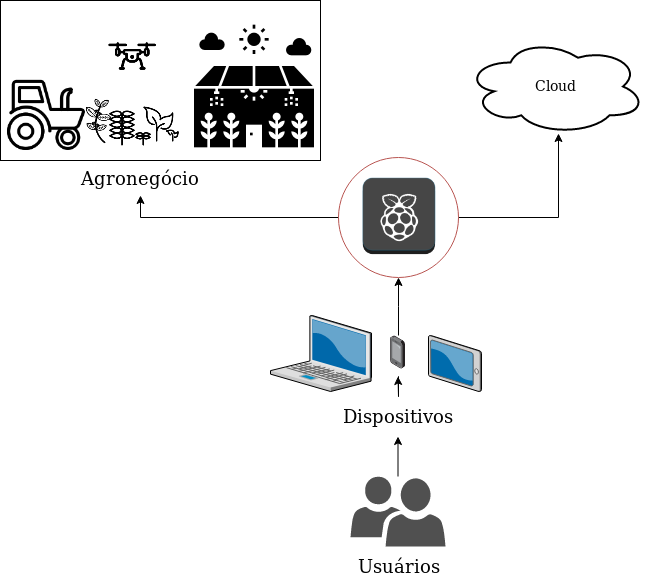
\includegraphics[scale=0.5]{novaimagem.png}
    \caption{Exemplo visual do comportamento da Raspberry PI 3 como nodo da névoa em aplicações de Agronegócio}
    \label{fig:my_label}
\end{figure}{}

Junto ao \textit{NDBench}, são disponibilizadas as configurações das tabelas dos bancos de dados necessárias para que estejam aptos a receber a simulação. Logo, o Cassandra foi configurado de acordo, sendo criado somente um único nodo, o qual julgamos já ser suficiente para testar o desempenho do dispositivo.  

A comunicação entre as máquinas foi realizada por canal criado pelas portas \textit{ethernet}, via cabo de rede, de forma a diminuir o ruído nos resultados obtidos. A configuração da máquina cliente manteve as configurações \textit{default}, ou seja, alguns valores pré selecionados pelo simulador foram mantidos. Somente opções como \textit{numWrites / numReads} e \textit{writeRateLimit / readRateLimit} foram alteradas, como demonstrado na Tabela 2, de forma a alcançar um \textit{benchmark} no qual fosse possível chegar próximo a um limite do dispositivo e analisar um real cenário de aplicação.  

\begin{table}[!ht]
\centering
\caption{Valores atribuídos às variáveis de execução do \textit{NDBench} durante os diferentes experimentos executados.}
\begin{tabular}{c|ccc}
\multirow{2}{*}{\textbf{Parâmetro}} & \multicolumn{3}{c}{\textbf{Valores atribuídos}}                                                                    \\ \cline{2-4} 
                                    & \multicolumn{1}{c|}{\textbf{Experimento 1}} & \multicolumn{1}{c|}{\textbf{Experimento 2}} & \textbf{Experimento 3} \\ \hline
numWrite                            & \multicolumn{1}{c|}{256 Threads}            & \multicolumn{1}{c|}{256 Threads}            & 256 Threads            \\ \hline
numRead                             & \multicolumn{1}{c|}{256 Threads}            & \multicolumn{1}{c|}{256 Threads}            & 256 Threads            \\ \hline
writeRateLimit                      & \multicolumn{1}{c|}{2.000 e/s}              & \multicolumn{1}{c|}{0 e/s}                  & 500 e/s                \\ \hline
readRateLimit                       & \multicolumn{1}{c|}{0 l/s}                  & \multicolumn{1}{c|}{2.000 l/s}              & 1.500 l/s              \\ \hline
\end{tabular}
\end{table}

Todos os experimentos contaram com a duração de 25 minutos, sem sofrer alteração na configuração do simulador durante a execução, embora o simulador nos permitisse isso. Experimentos foram executados anteriormente para analisar as possíveis variações, cargas e falhas dada pelo simulador, não sofrendo variações, empregou-se cargas aproximadas do limite de resposta da Raspberry Pi 3 para a obtenção dos resultados analisados na Seção \ref{sec:Resultados}. Com as cargas selecionadas, criaram-se três cenários, de forma a simular determinadas situações. Inicialmente realizamos um teste que simula somente escritas no banco, depois outro que simula somente leituras e, por fim, uma simulação onde ambos ocorrem, com 75\% de leituras e 25\% de escritas.

Para execuções mais precisas, fizemos uso de \textit{scripts python} para realizar as operações necessárias para execução do simulador pois, como o simulador fornece a interface de usuário, o inicio poderia ser dado por meio dela, porém a inicialização e finalização não seriam precisas. Dado que o simulador permite a sua utilização via linha de comando com chamadas \textit{curl}, optou-se por automatizar essa parte. Todo o roteiro de testes e os arquivos necessários aqui apresentados estão disponíveis no GitHub\footnote{GitHub: \url{github.com/SouzaGuilherme/research\_PI3\_evaluate\_experiment}}.

\section{Resultados} \label{sec:Resultados}

Após a análise dos resultados obtidos a partir da execução do simulador nos cenários criados, focamos nos resultados de latência nos percentis 95 e 99, latência média e requisições por segundo. Para uma melhor visualização dos resultados, desconsideramos o tempo de lançamento do simulador. Todos os resultados, incluindo os tempos de lançamento, estão disponíveis para consulta no GitHub\footnote{GitHub: \url{github.com/SouzaGuilherme/research_PI3_evaluate_experiment}} junto aos fontes.

A escolha em demonstrar os resultados não somente em latência média, mas também em percentil 95 e 99 vem das informações que a média nos esconde, sendo atualmente a métrica mais utilizada em servidores. Logo, com isso temos resultados como 95\% dos usuários são atendidos abaixo de uma certa latência, ou seja, o servidor pode estar atendendo alguns usuários com um latência ruim e isso variará com a quantidade de usuários que o servidor esta atendendo (o mesmo ocorre ao utilizar o percentil 99).

\begin{table}[!hb]
\centering
\caption{Total de escritas e leituras alcançadas com sucesso e falhas ao final de 25 minutos. \label{tab:usa}}
\begin{tabular}{c|c|c|cc}
\multirow{2}{*}{\textbf{Experimentos}} & \multicolumn{2}{c|}{\textbf{Escrita}} & \multicolumn{2}{c}{\textbf{Leitura}}                   \\ \cline{2-5} 
                                      & \textbf{Sucesso}   & \textbf{Falha}   & \multicolumn{1}{c|}{\textbf{Sucesso}} & \textbf{Falha} \\ \hline
Experimento 1                         & 1.990.963          & 2.585            & \multicolumn{1}{c|}{-}                & -              \\ \hline
Experimento 2                         & -                  & -                & \multicolumn{1}{c|}{2.155.112}        & 0              \\ \hline
Experimento 3                         & 834.606            & 26               & \multicolumn{1}{c|}{808.983}          & 0              \\ \hline
\end{tabular}
\end{table}

Podemos observar, na Tabela \ref{tab:usa}, o montante de operações realizadas durante os 25 minutos de execução do simulador, podendo ser visto que são alcançadas em torno de dois milhões de operações em ambos cenários. O Experimento 1 apresentou uma taxa de falhas em torno de $\pm$ 0.1298\%, enquanto os Experimentos 2 e 3 apresentaram zero e 26 falhas respectivamente, caindo em \textit{time out}, possivelmente pela demora da Raspberry Pi 3 em atender a demanda.

No primeiro cenário, no qual realizamos somente escritas, observou-se que a Raspberry atendia a demanda conforme sua capacidade, alcançando um atendimento de mais de 1.200 operações por segundo. Mantendo a latência média e a percentil 95 abaixo dos 500ms, essas informações estão contidas na Figura \ref{fig:avr-memmap} (a) e (b). 

\begin{figure}[!ht]
  \centering
  \mbox{%
    \subfigure[Latência de escritas]{\label{avr-prgmem}%
      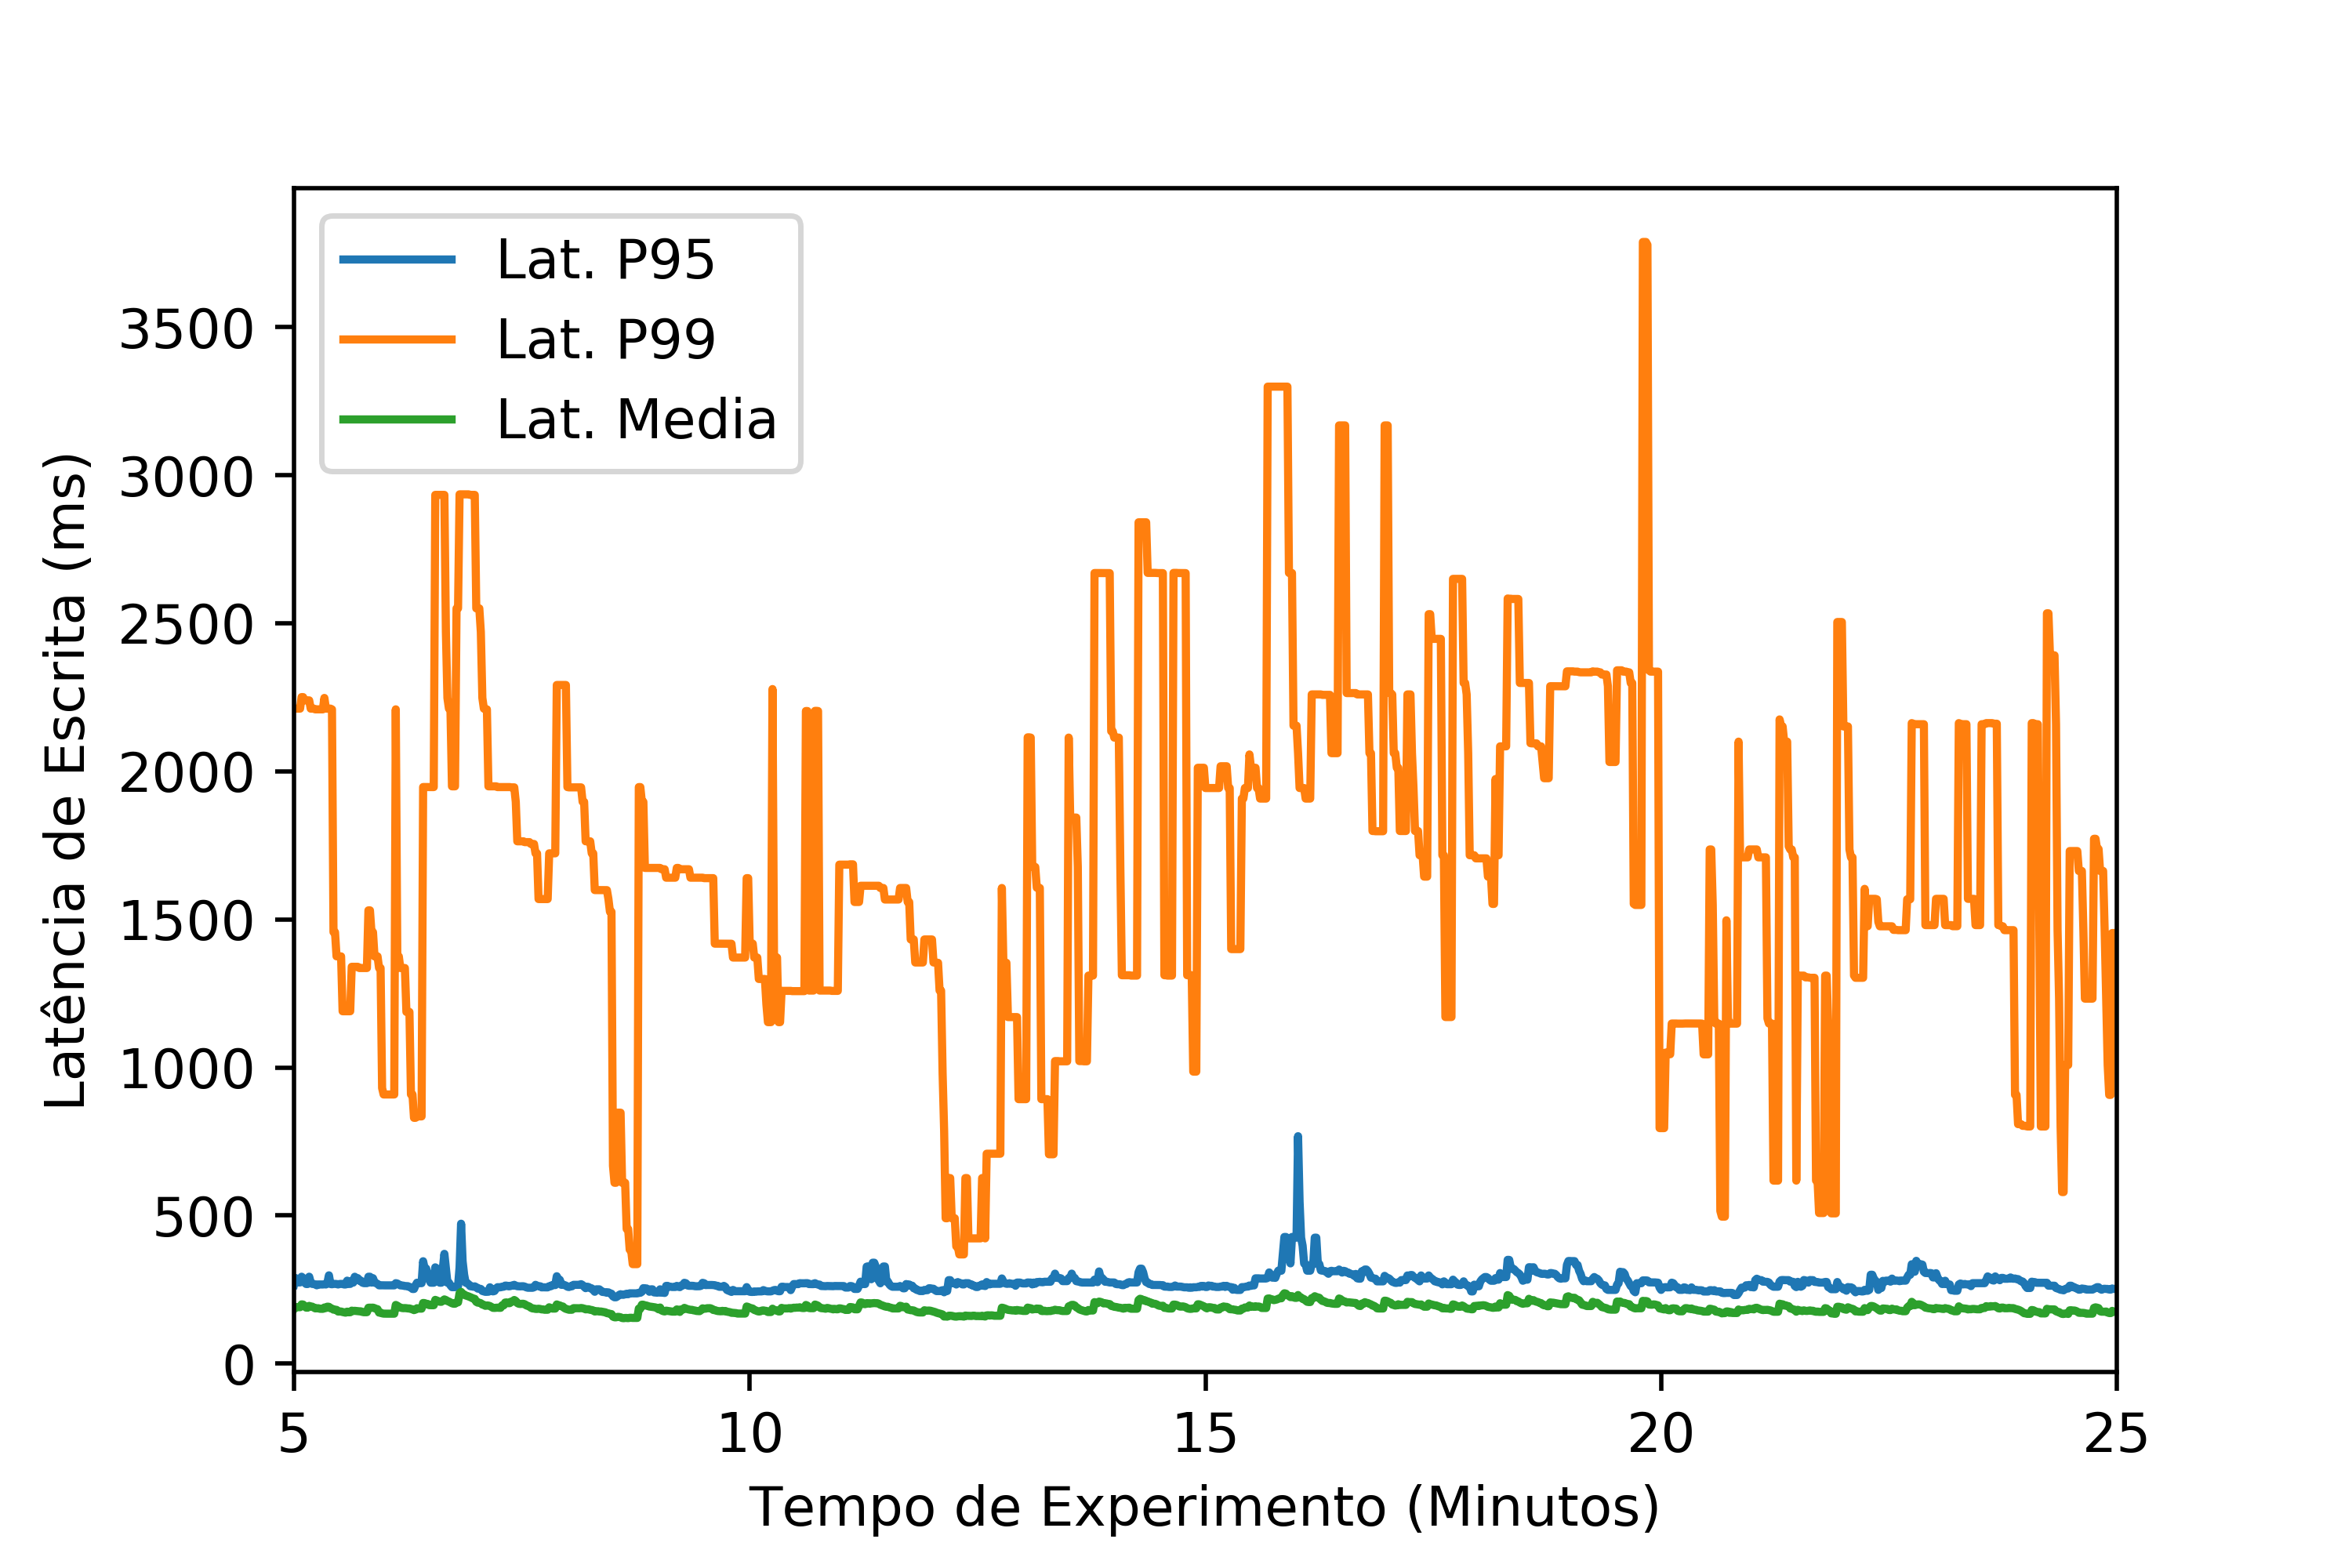
\includegraphics[width=0.5\textwidth]{PI3__SO-WRITE__LATENCIAS__2000W.png}}\qquad
    \subfigure[Requisições por segundo]{\label{avr-datamem}%
      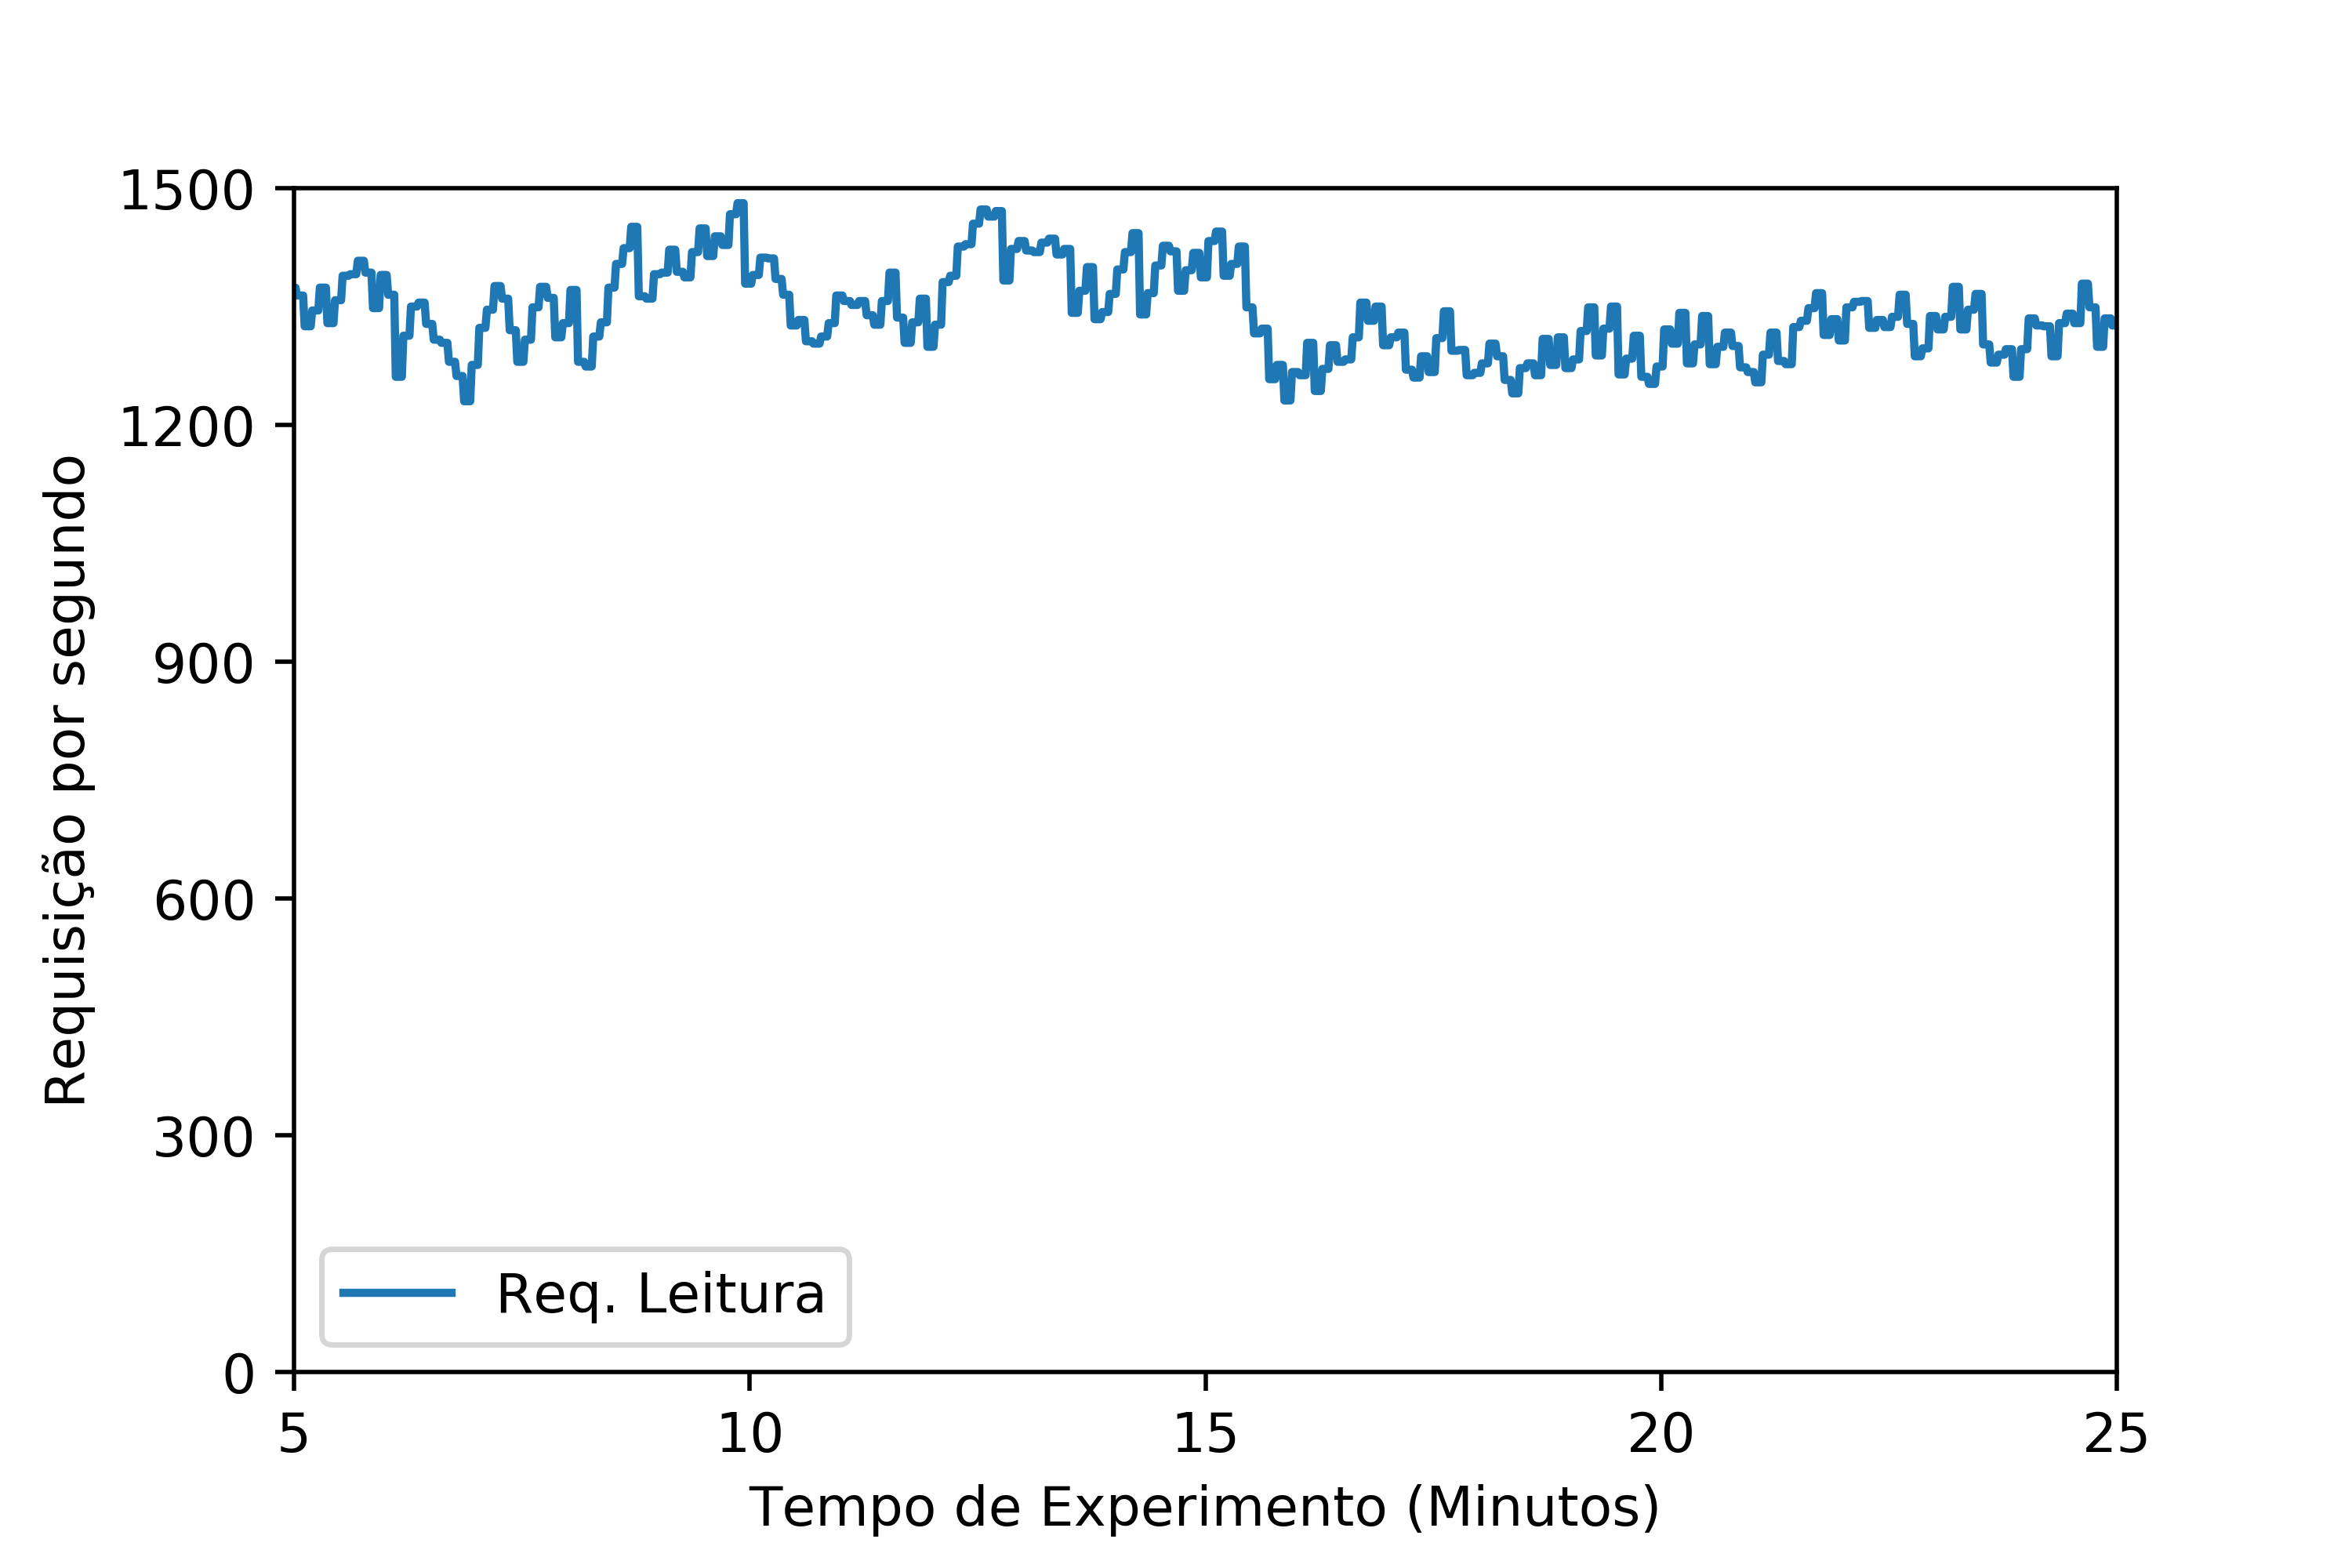
\includegraphics[width=0.5\textwidth]{PI3__RPS__SO-WRITE__2000W.png}}
    }
  \caption{Latências e requisições por segundo durante escrita no período de execução de 25 minutos desconsiderando os 5 primeiros do simulador.}
  \label{fig:avr-memmap}
\end{figure}

Onde havia somente leituras, a Raspberry Pi 3 demonstrou uma ótima desenvoltura, dado que conseguiu atender um número equivalente ao primeiro cenário em requisições por segundo entre 1.200 e 1.500 como pode ser visto na Figura \ref{fig:avr-memmap2} (b). Igualmente, manteve uma latência de qualidade como pode ser vista no Figura \ref{fig:avr-memmap2} (a), mantendo a média abaixo de 500ms e percentil 95 abaixo de 1000ms. 

\begin{figure}[!hb]
  \centering
  \mbox{%
    \subfigure[Latências de leituras]{\label{avr-prgmem2}%
      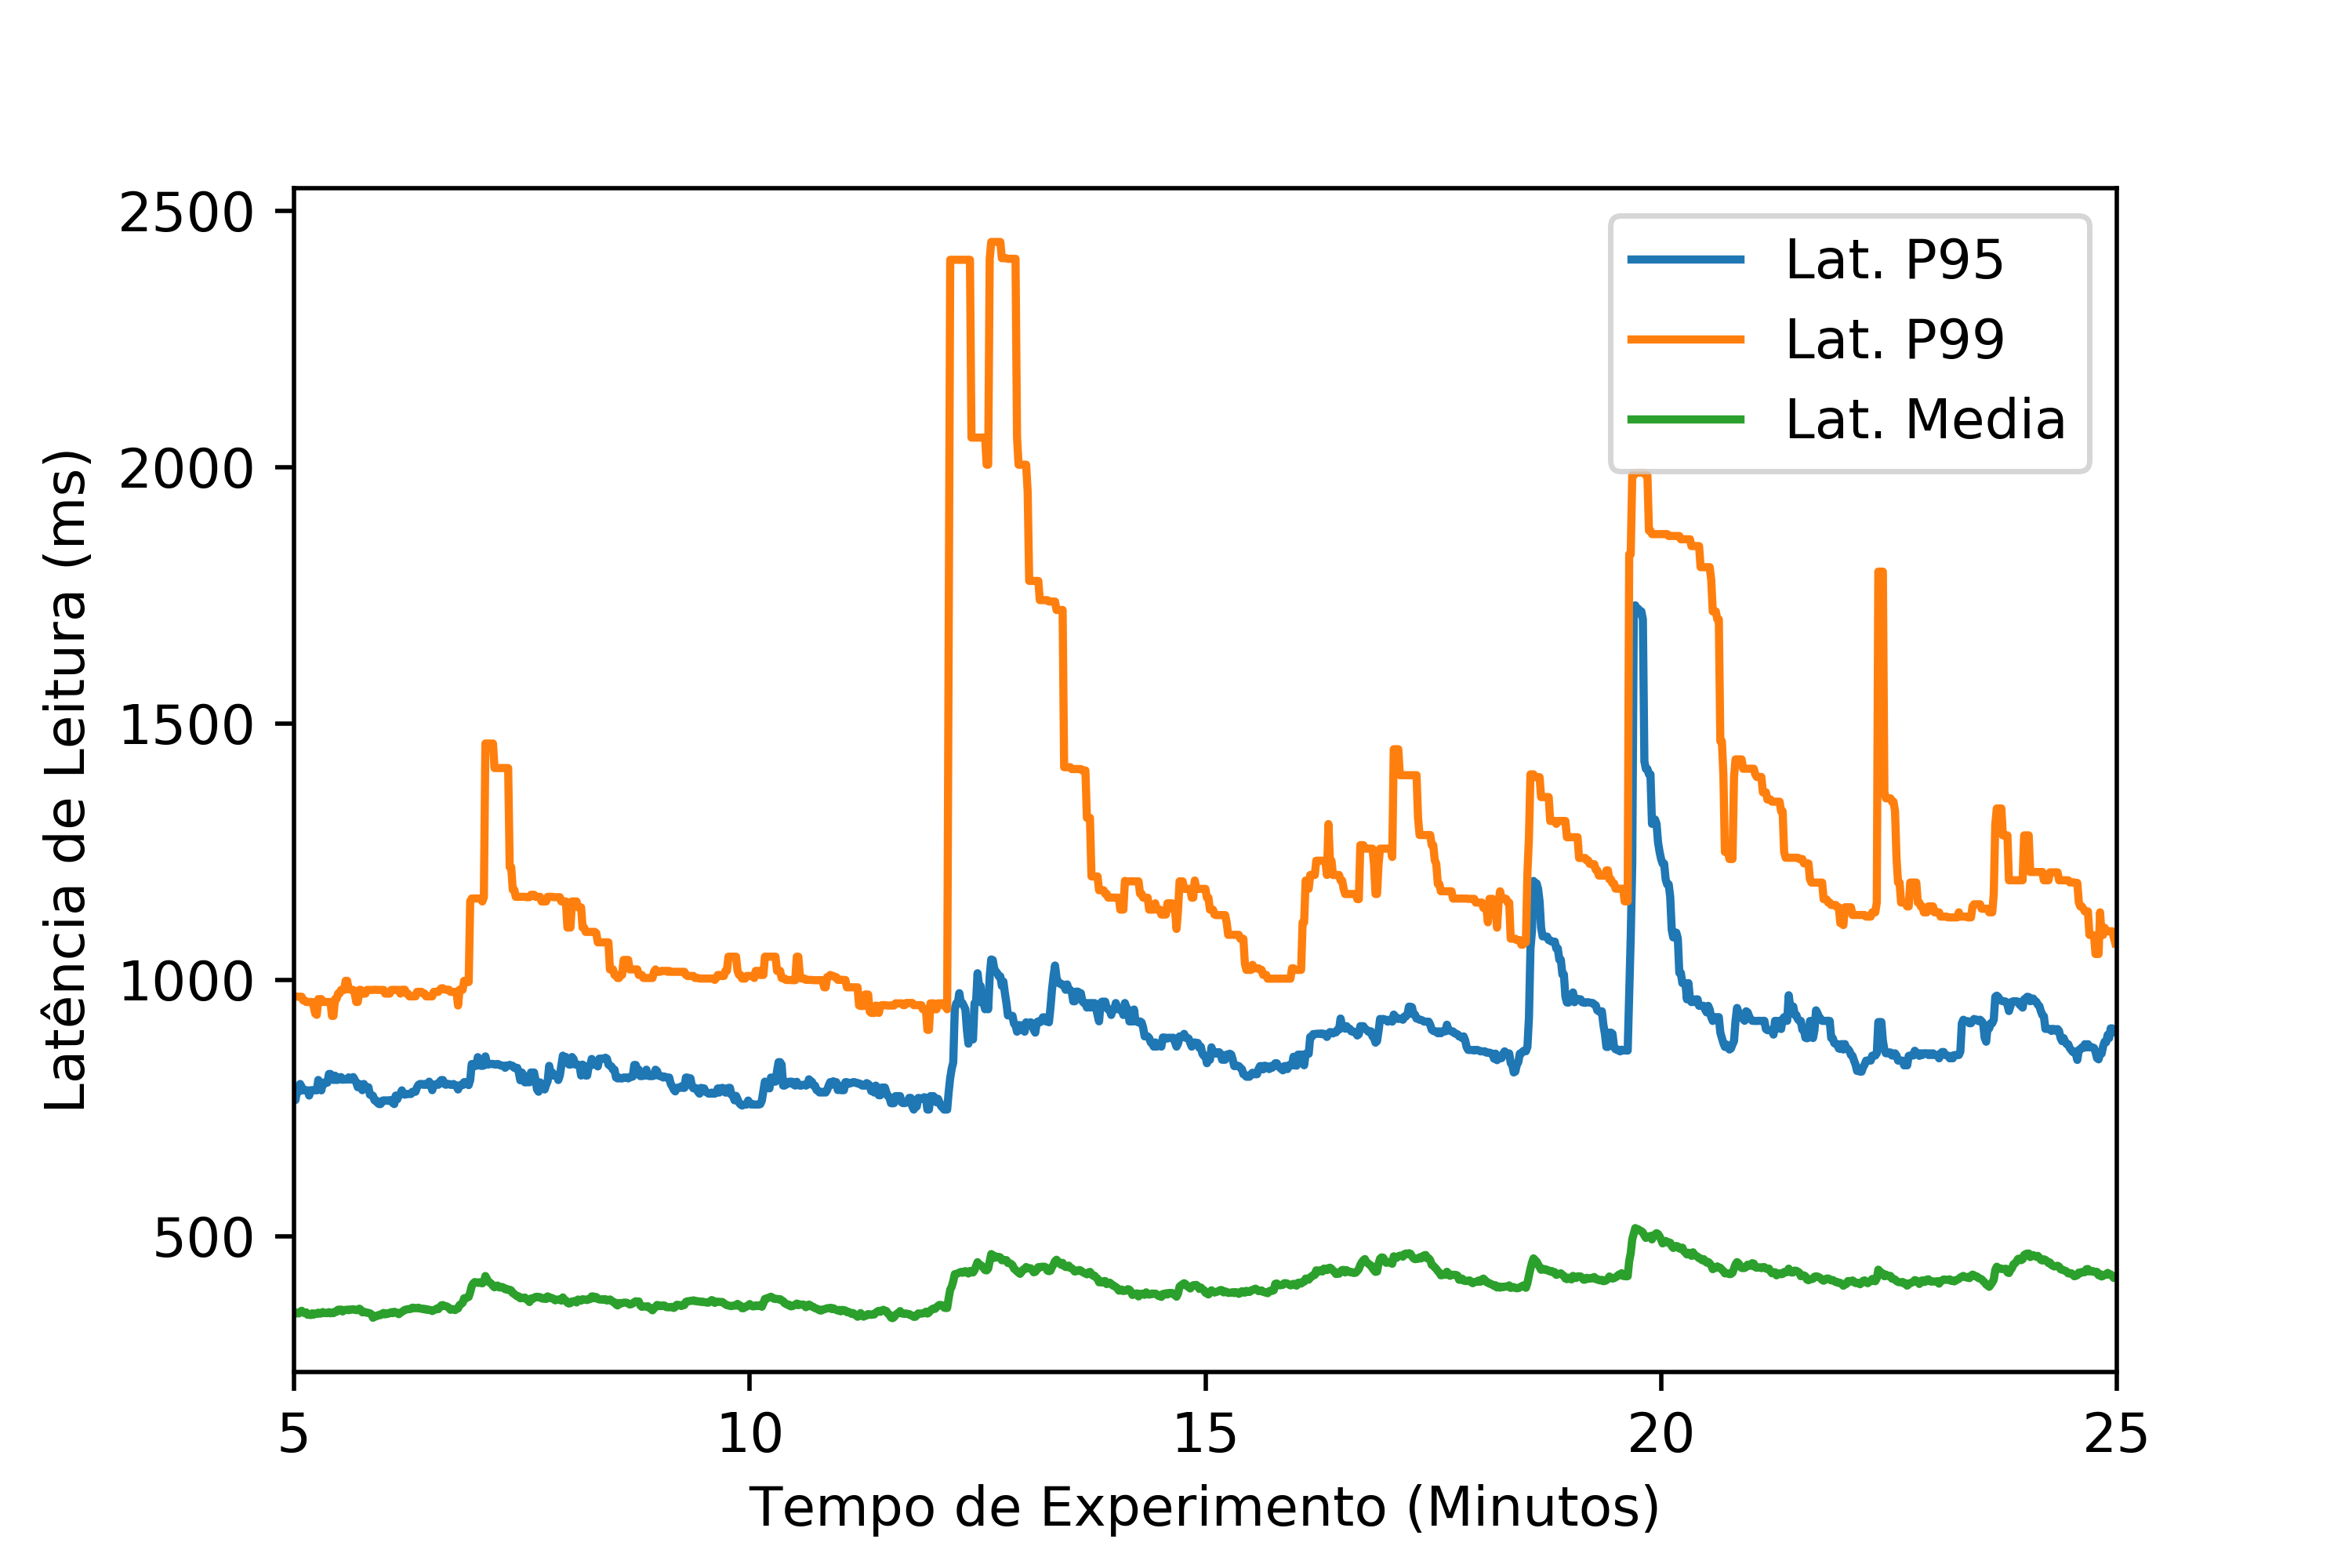
\includegraphics[width=0.5\textwidth]{PI3__SO-READ__LATENCIAS__2000W.png}}\qquad
    \subfigure[Operações por segundo]{\label{avr-datamem2}%
      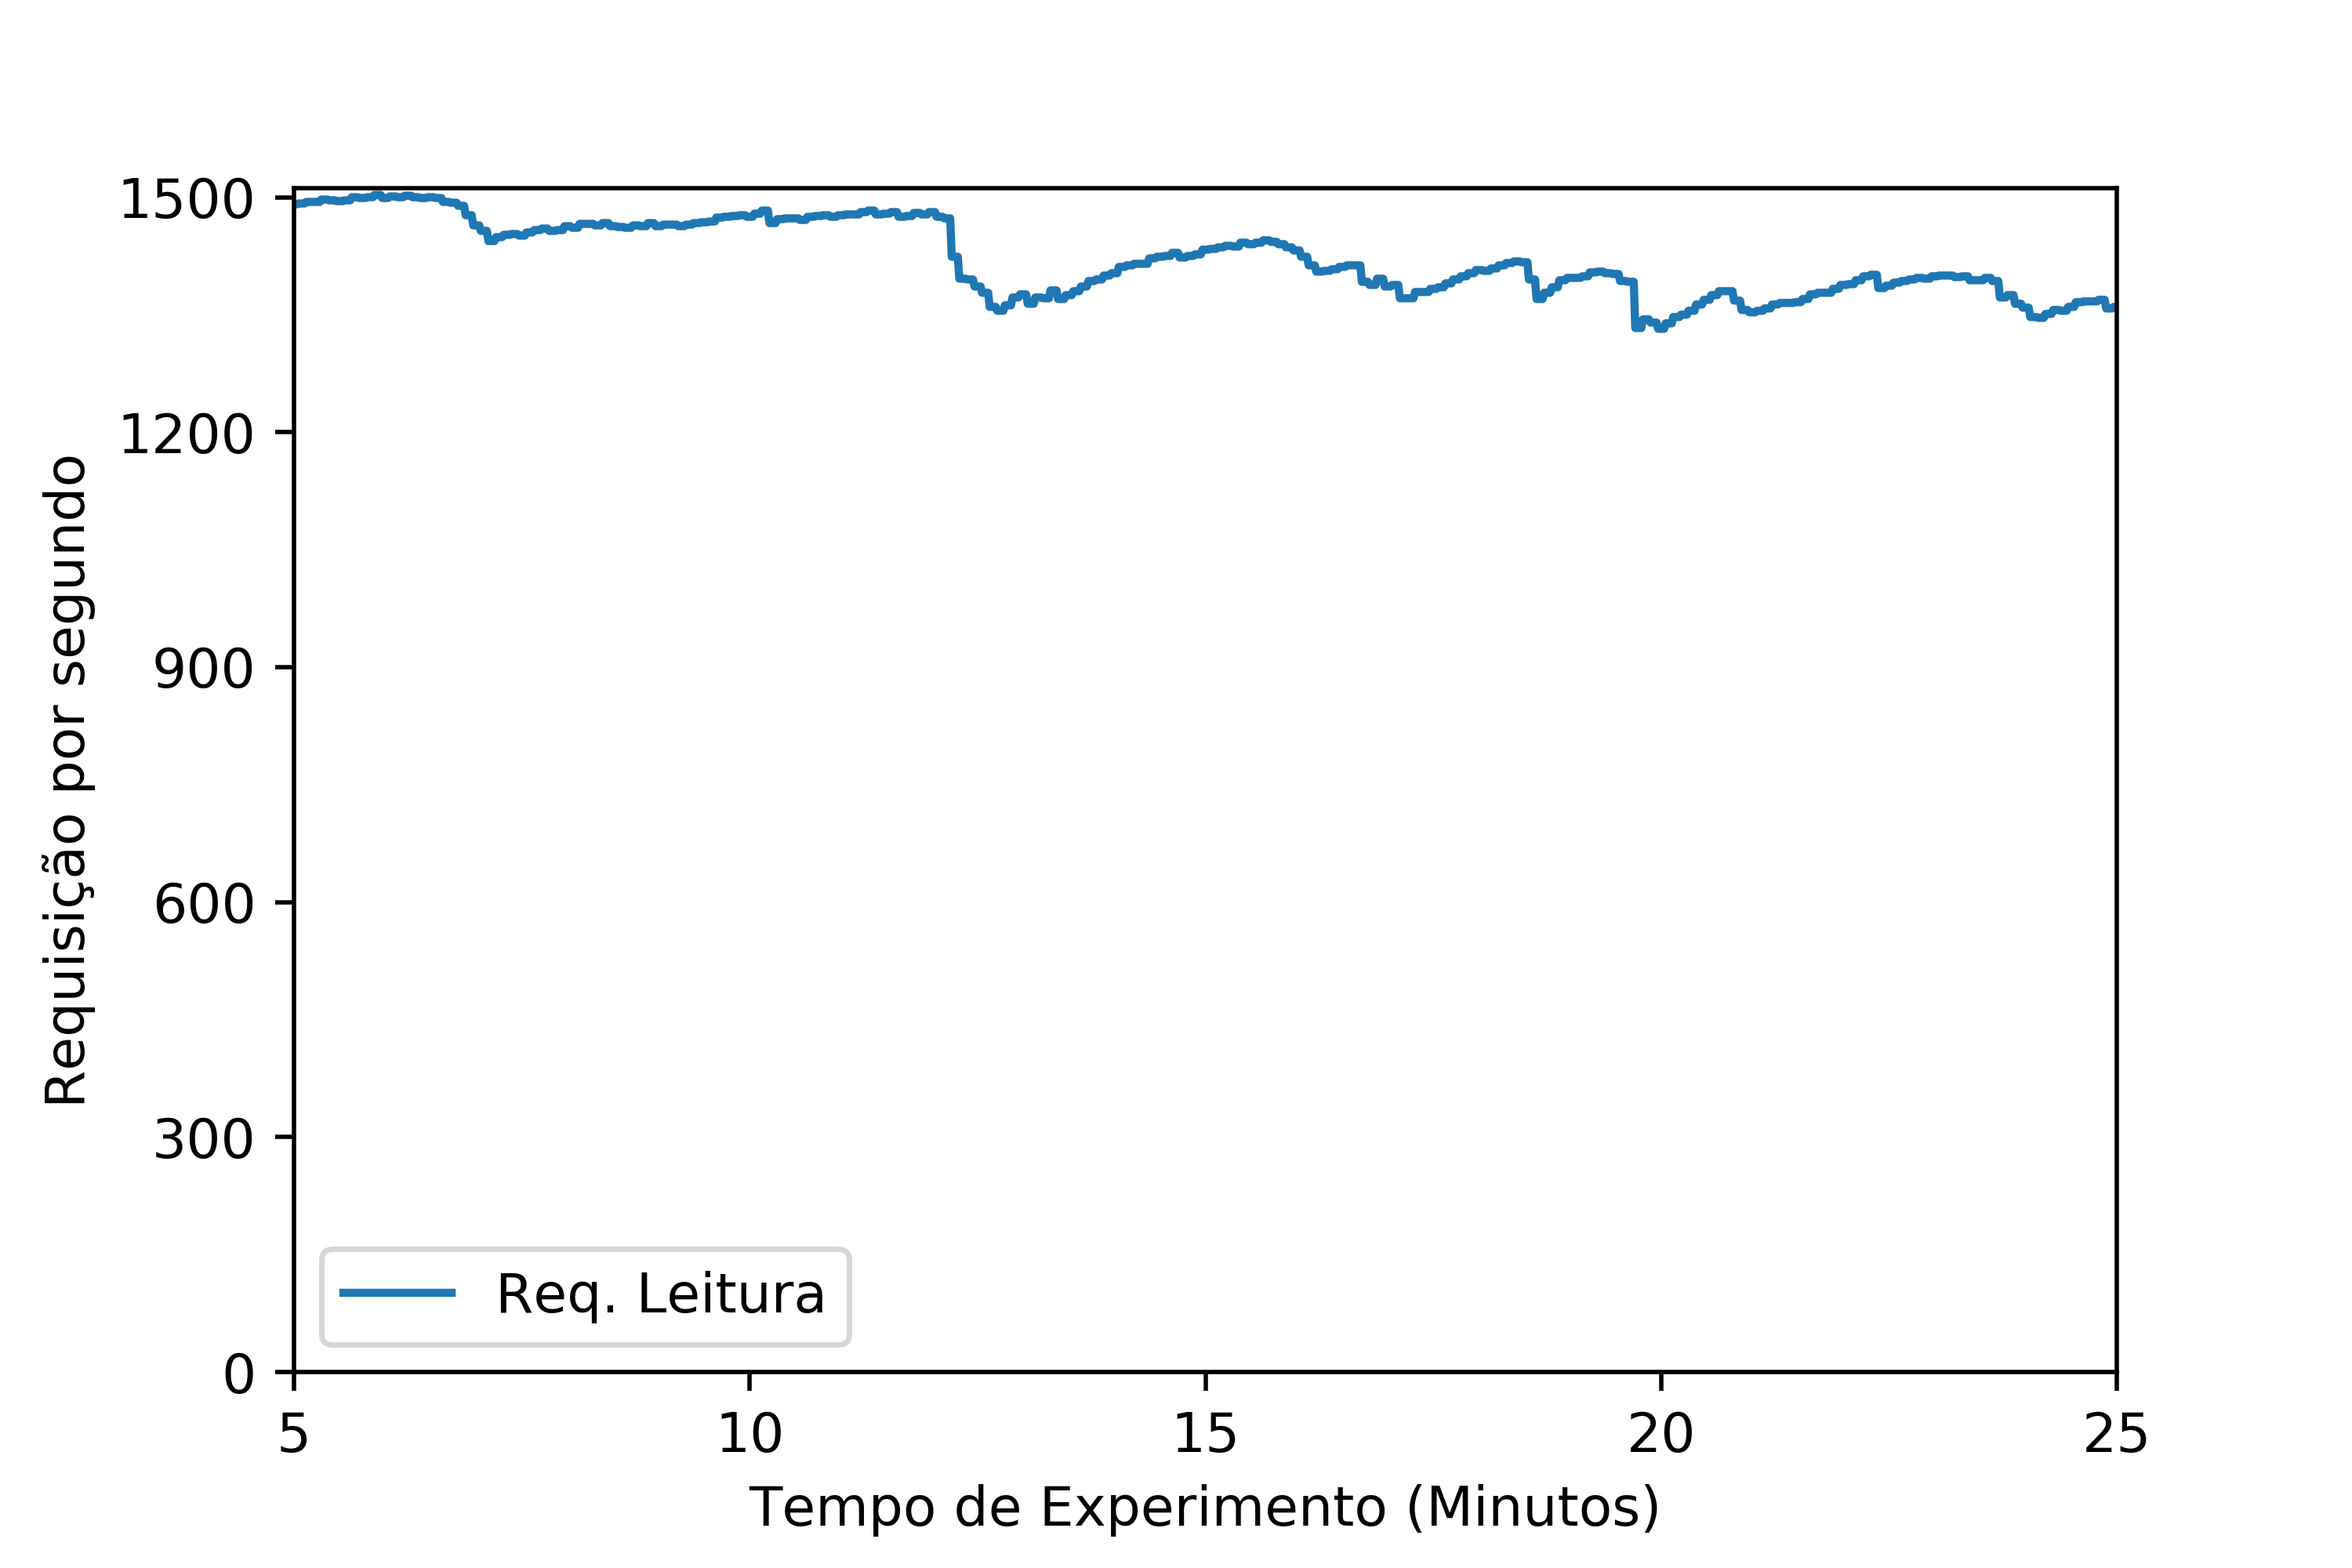
\includegraphics[width=0.5\textwidth]{PI3__RPS__SO-READ__2000W.png}}
    }
  \caption{Latências e requisições por segundo durante leitura no período de execução de 25 minutos desconsiderando os 5 iniciais do simulador.}
  \label{fig:avr-memmap2}
\end{figure}

Dados os resultados anteriores, alguns valores já eram esperados neste último cenário proposto, conforme pode-se observar na Figura \ref{fig:avr-memmap3} (a) e (b). Neste cenário mais realista de escritas e leituras simultâneas, a \textit{small board} manteve a qualidade no serviço, mesmo realizando ambas operações. Demonstrou uma baixa latência, tanto em percentil 95 estando um pouco a mais de 500ms, quanto a média, que como nos outros testes se manteve abaixo dos 500ms. Ao olharmos para as operações que realizou durante o período de execução do simulador, podemos ver que chegava em torno de mais de 450 requisições por segundo de escritas e leituras, como demonstrado na Figura \ref{fig:avr-memmap3} (c). Visto que nos resultados anteriores os alcances em requisições foram maiores, pudemos observar que a placa tenta distribuir igualmente o trabalho de forma a atender ambas necessidades.

\begin{figure}[!ht]
  \centering
  \mbox{%
    \subfigure[Latências de escritas]{\label{avr-prgmem3a}%
      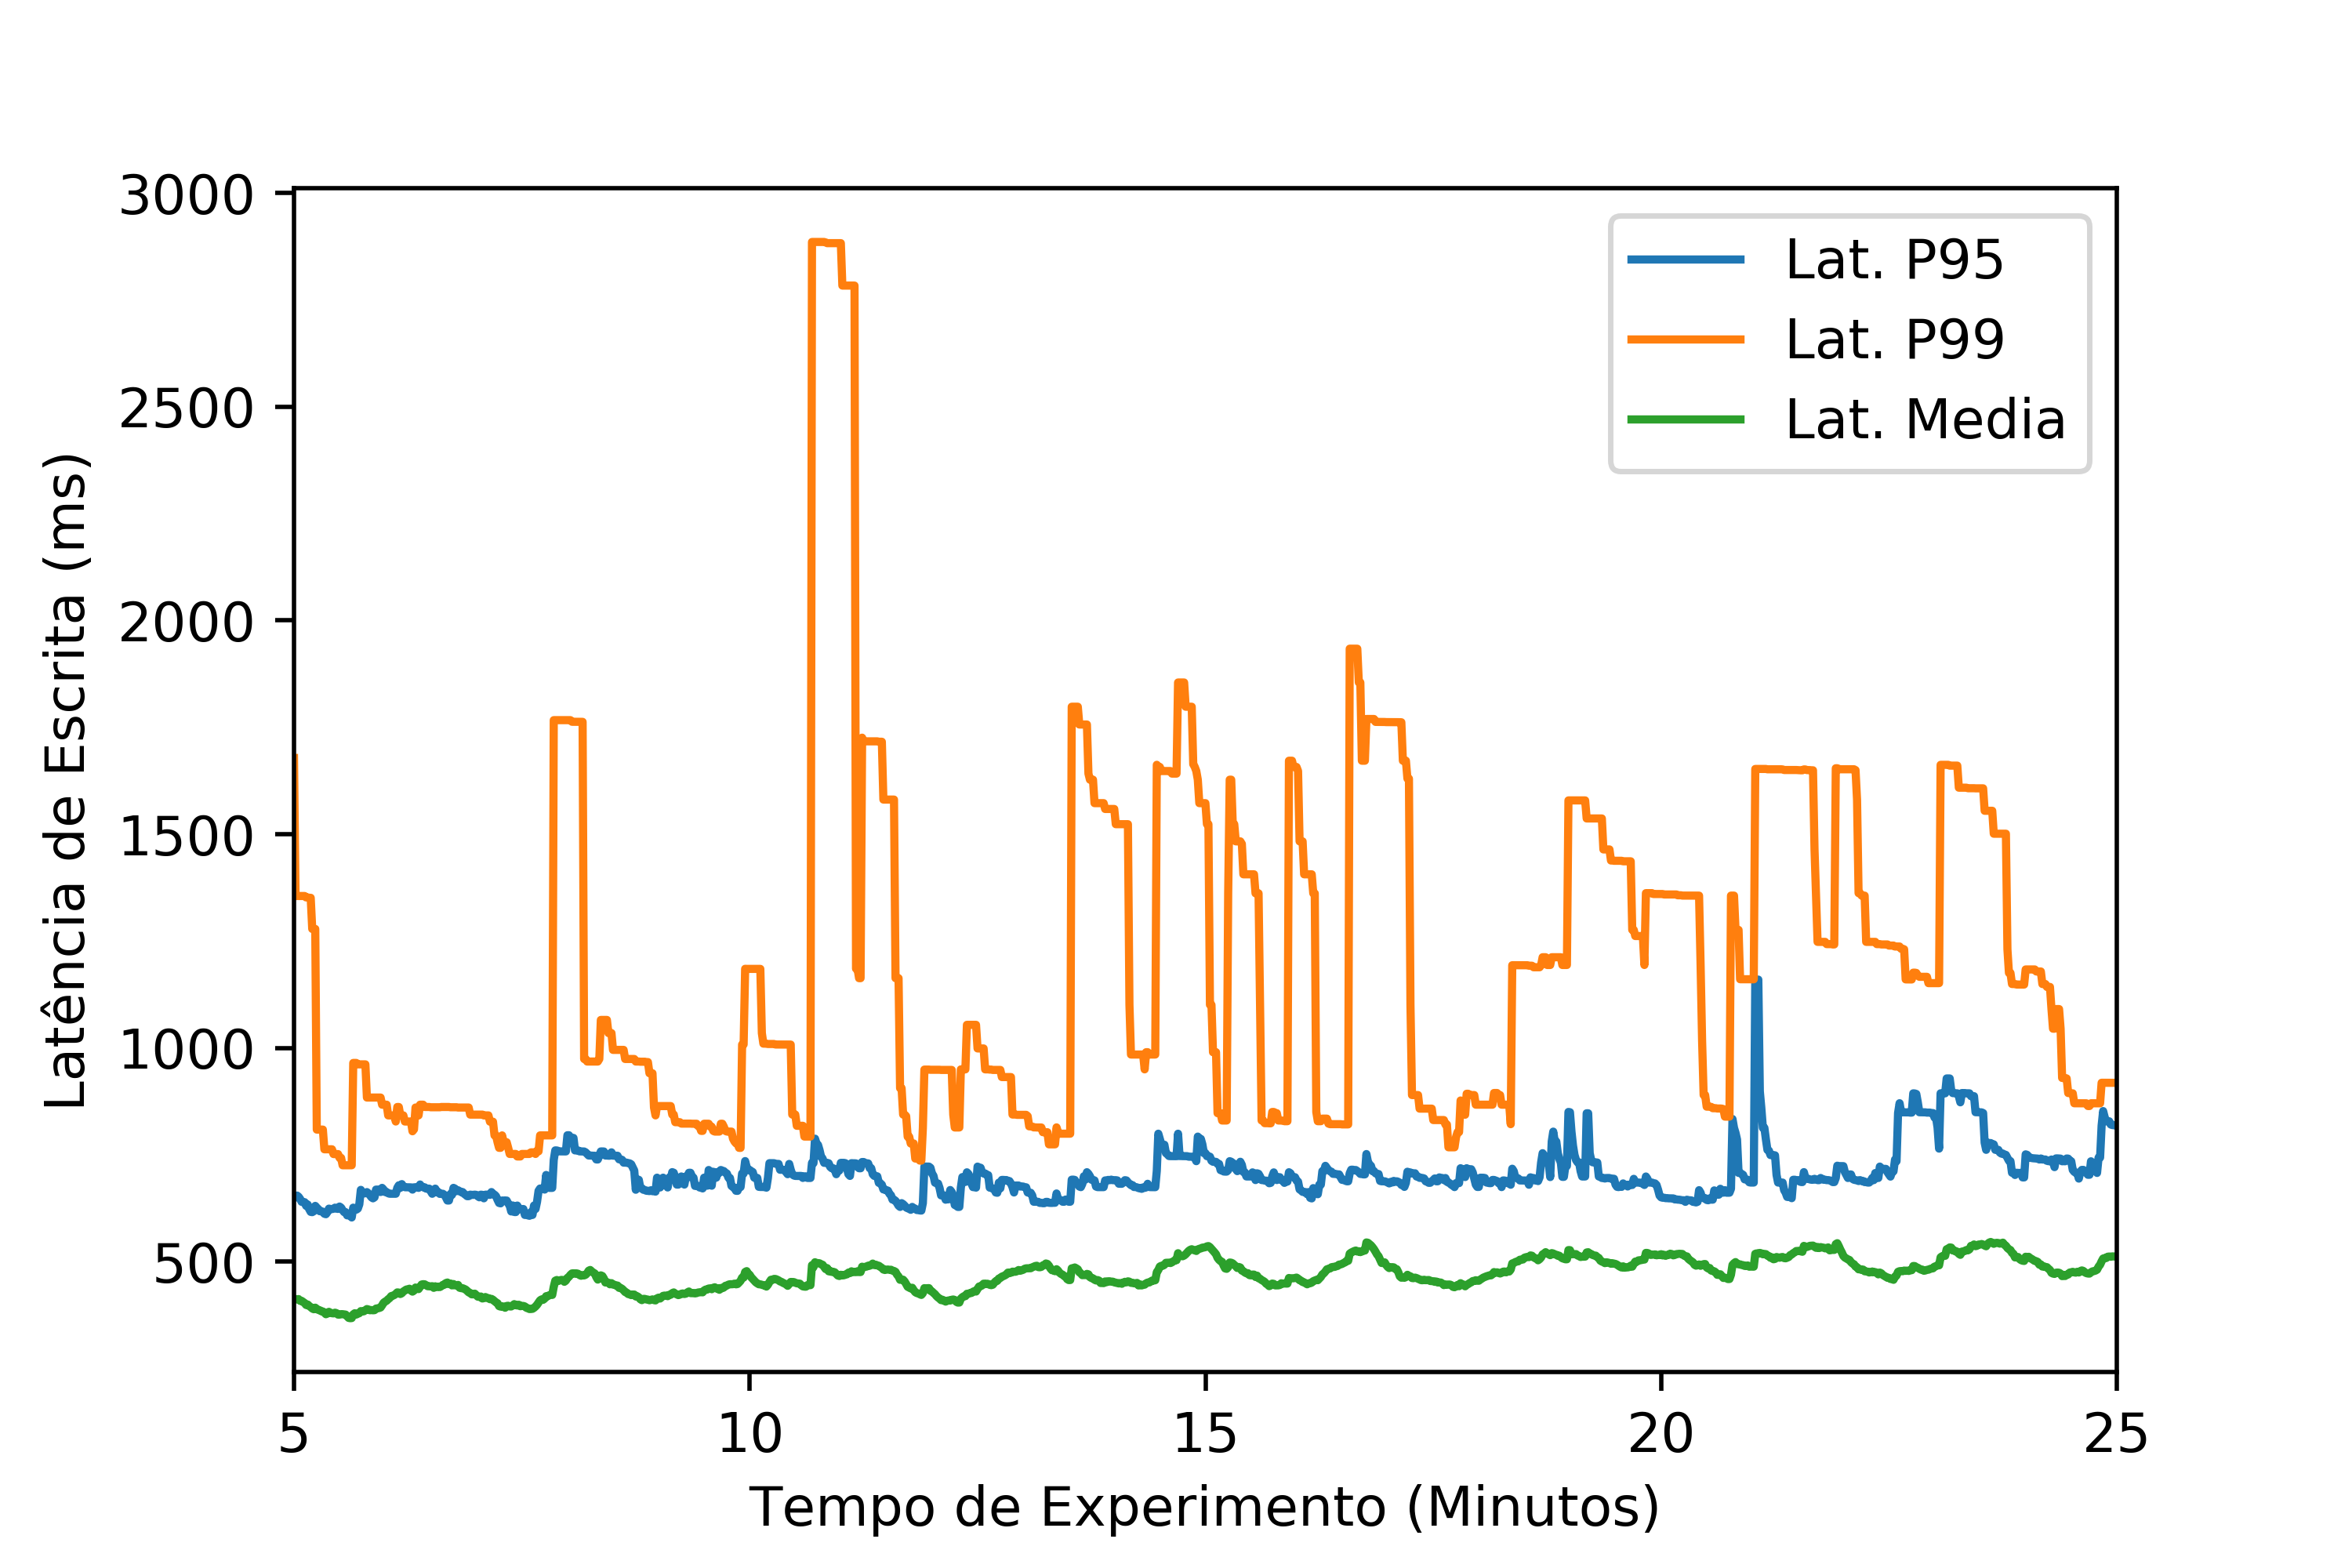
\includegraphics[width=0.5\textwidth]{PI3__WRITE__READ-WRITE__LATENCIAS__500W-1500R.png}}\qquad
    \subfigure[Latências de leituras]{\label{avr-prgmem3b}%
      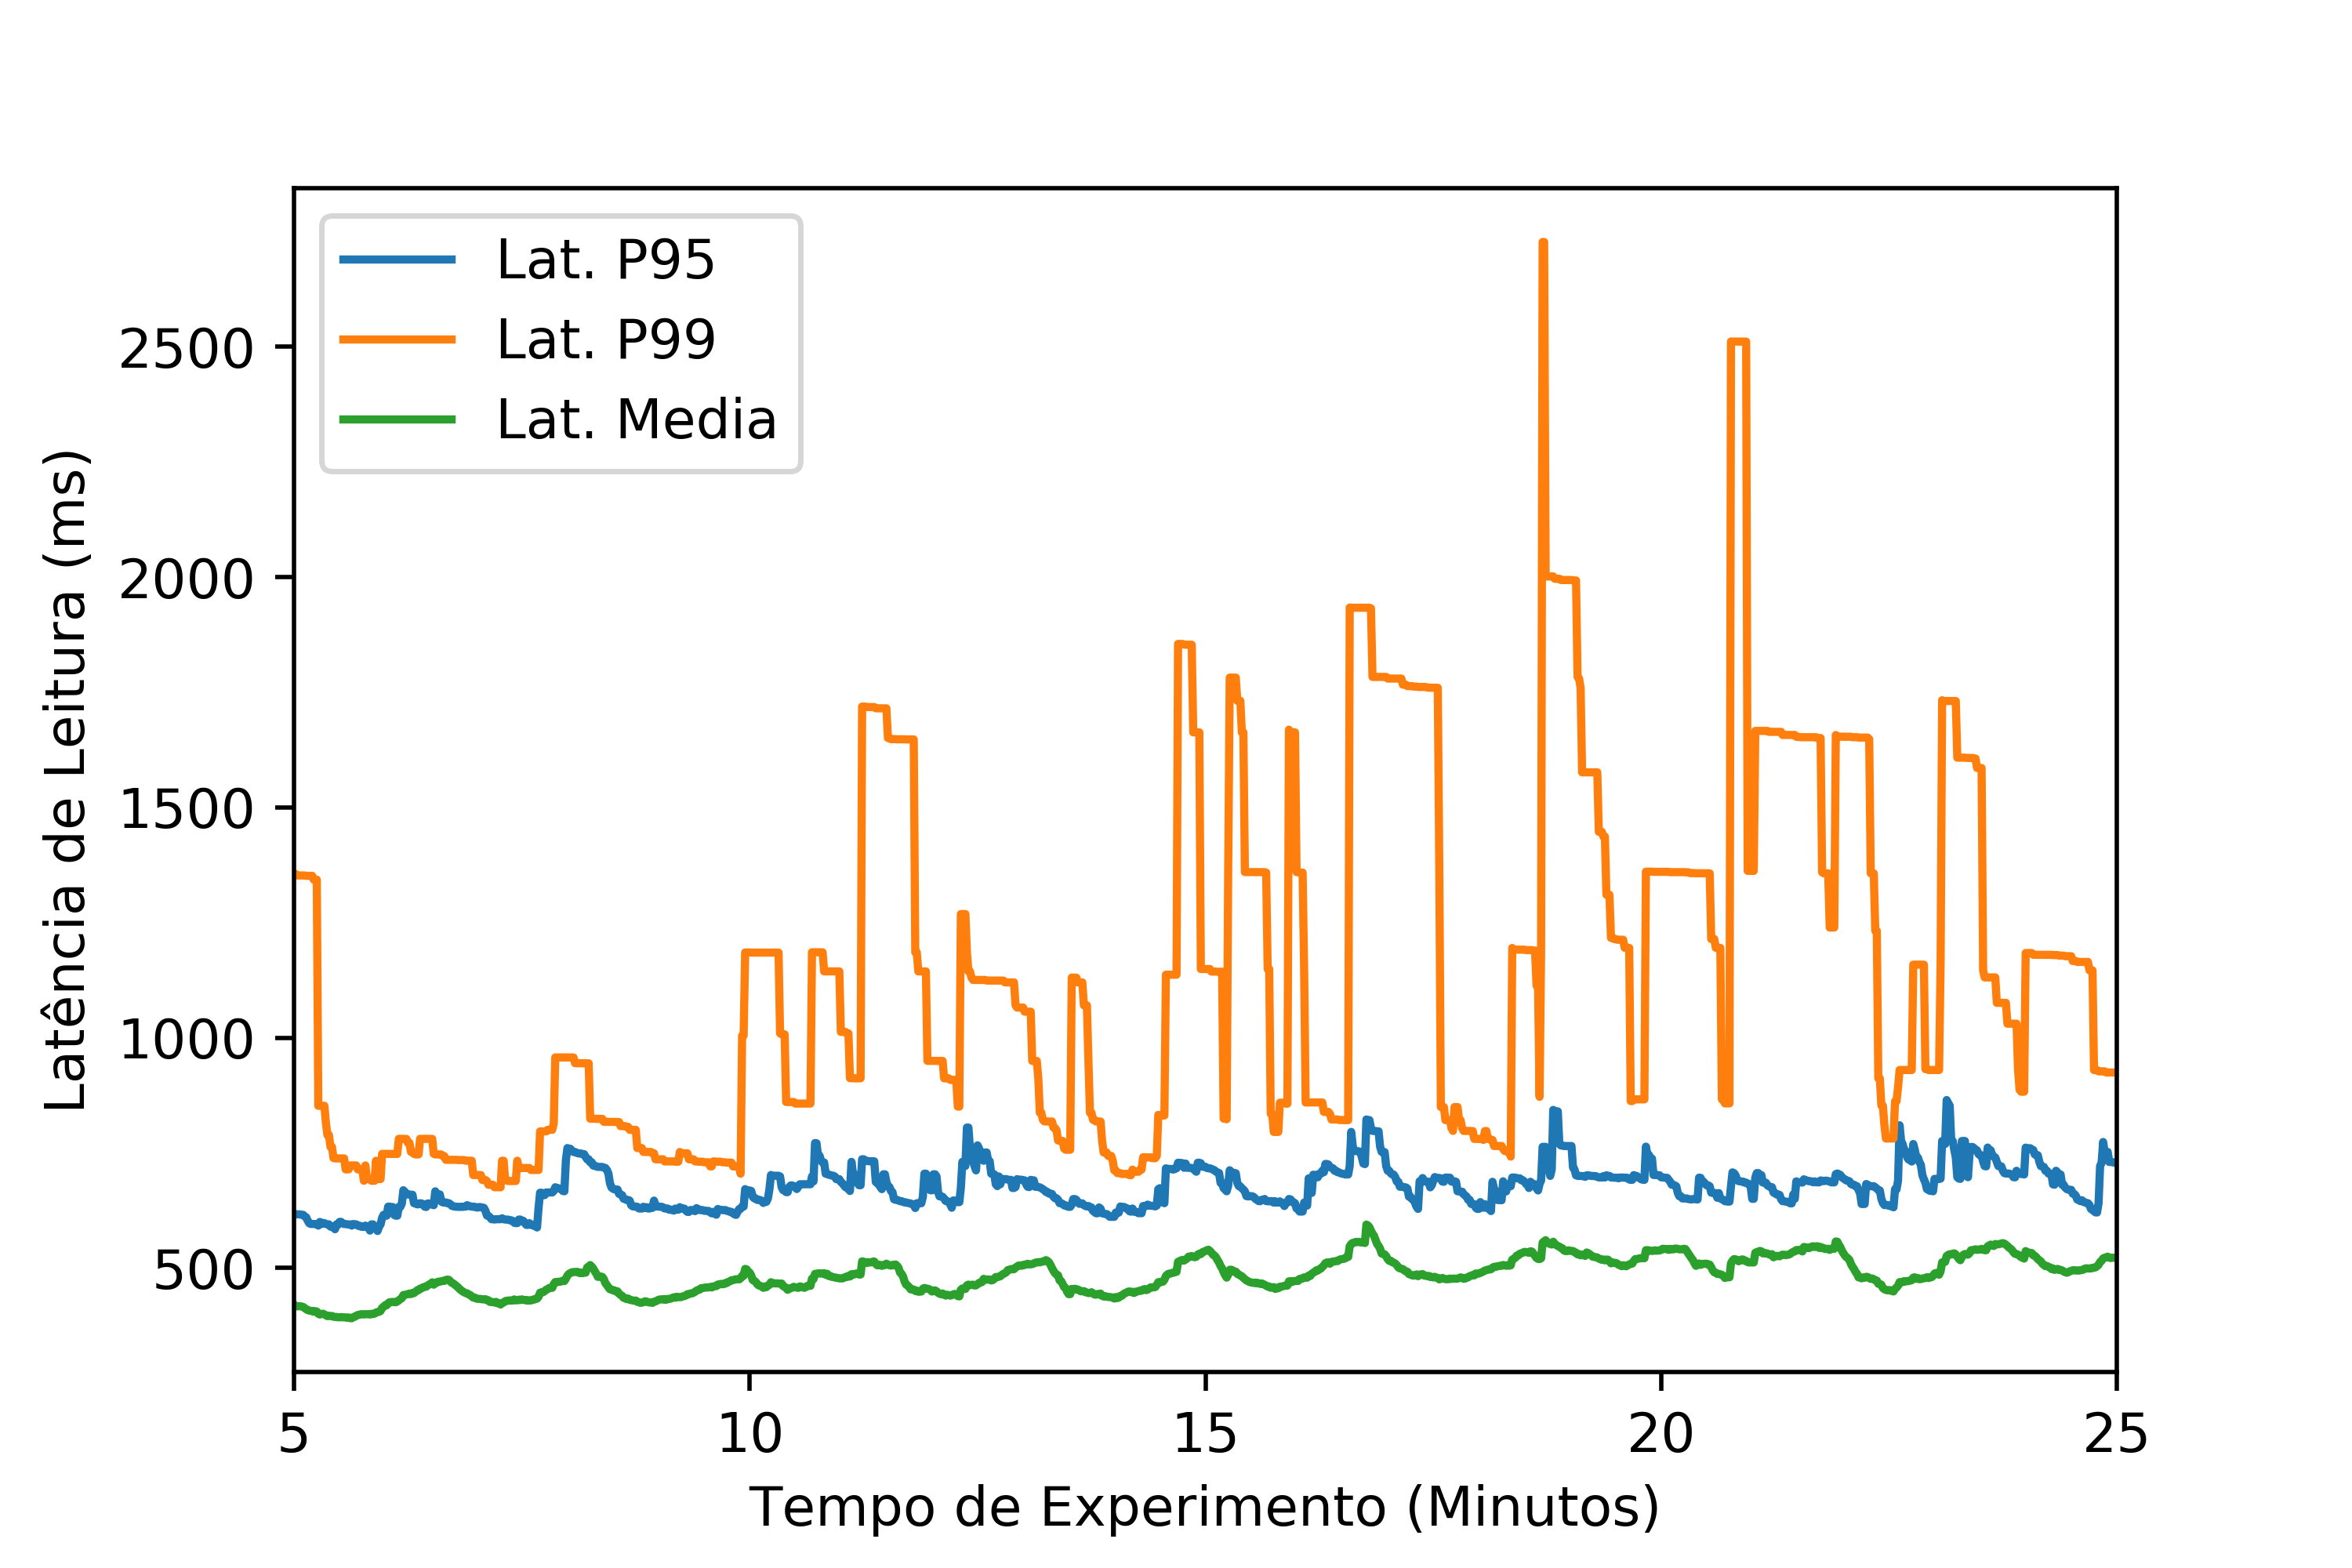
\includegraphics[width=0.5\textwidth]{PI3__READ__READ-WRITE__LATENCIAS__500W-1500R.png}}
    }
    \subfigure[Operações por segundo]{\label{avr-datamem3}%
      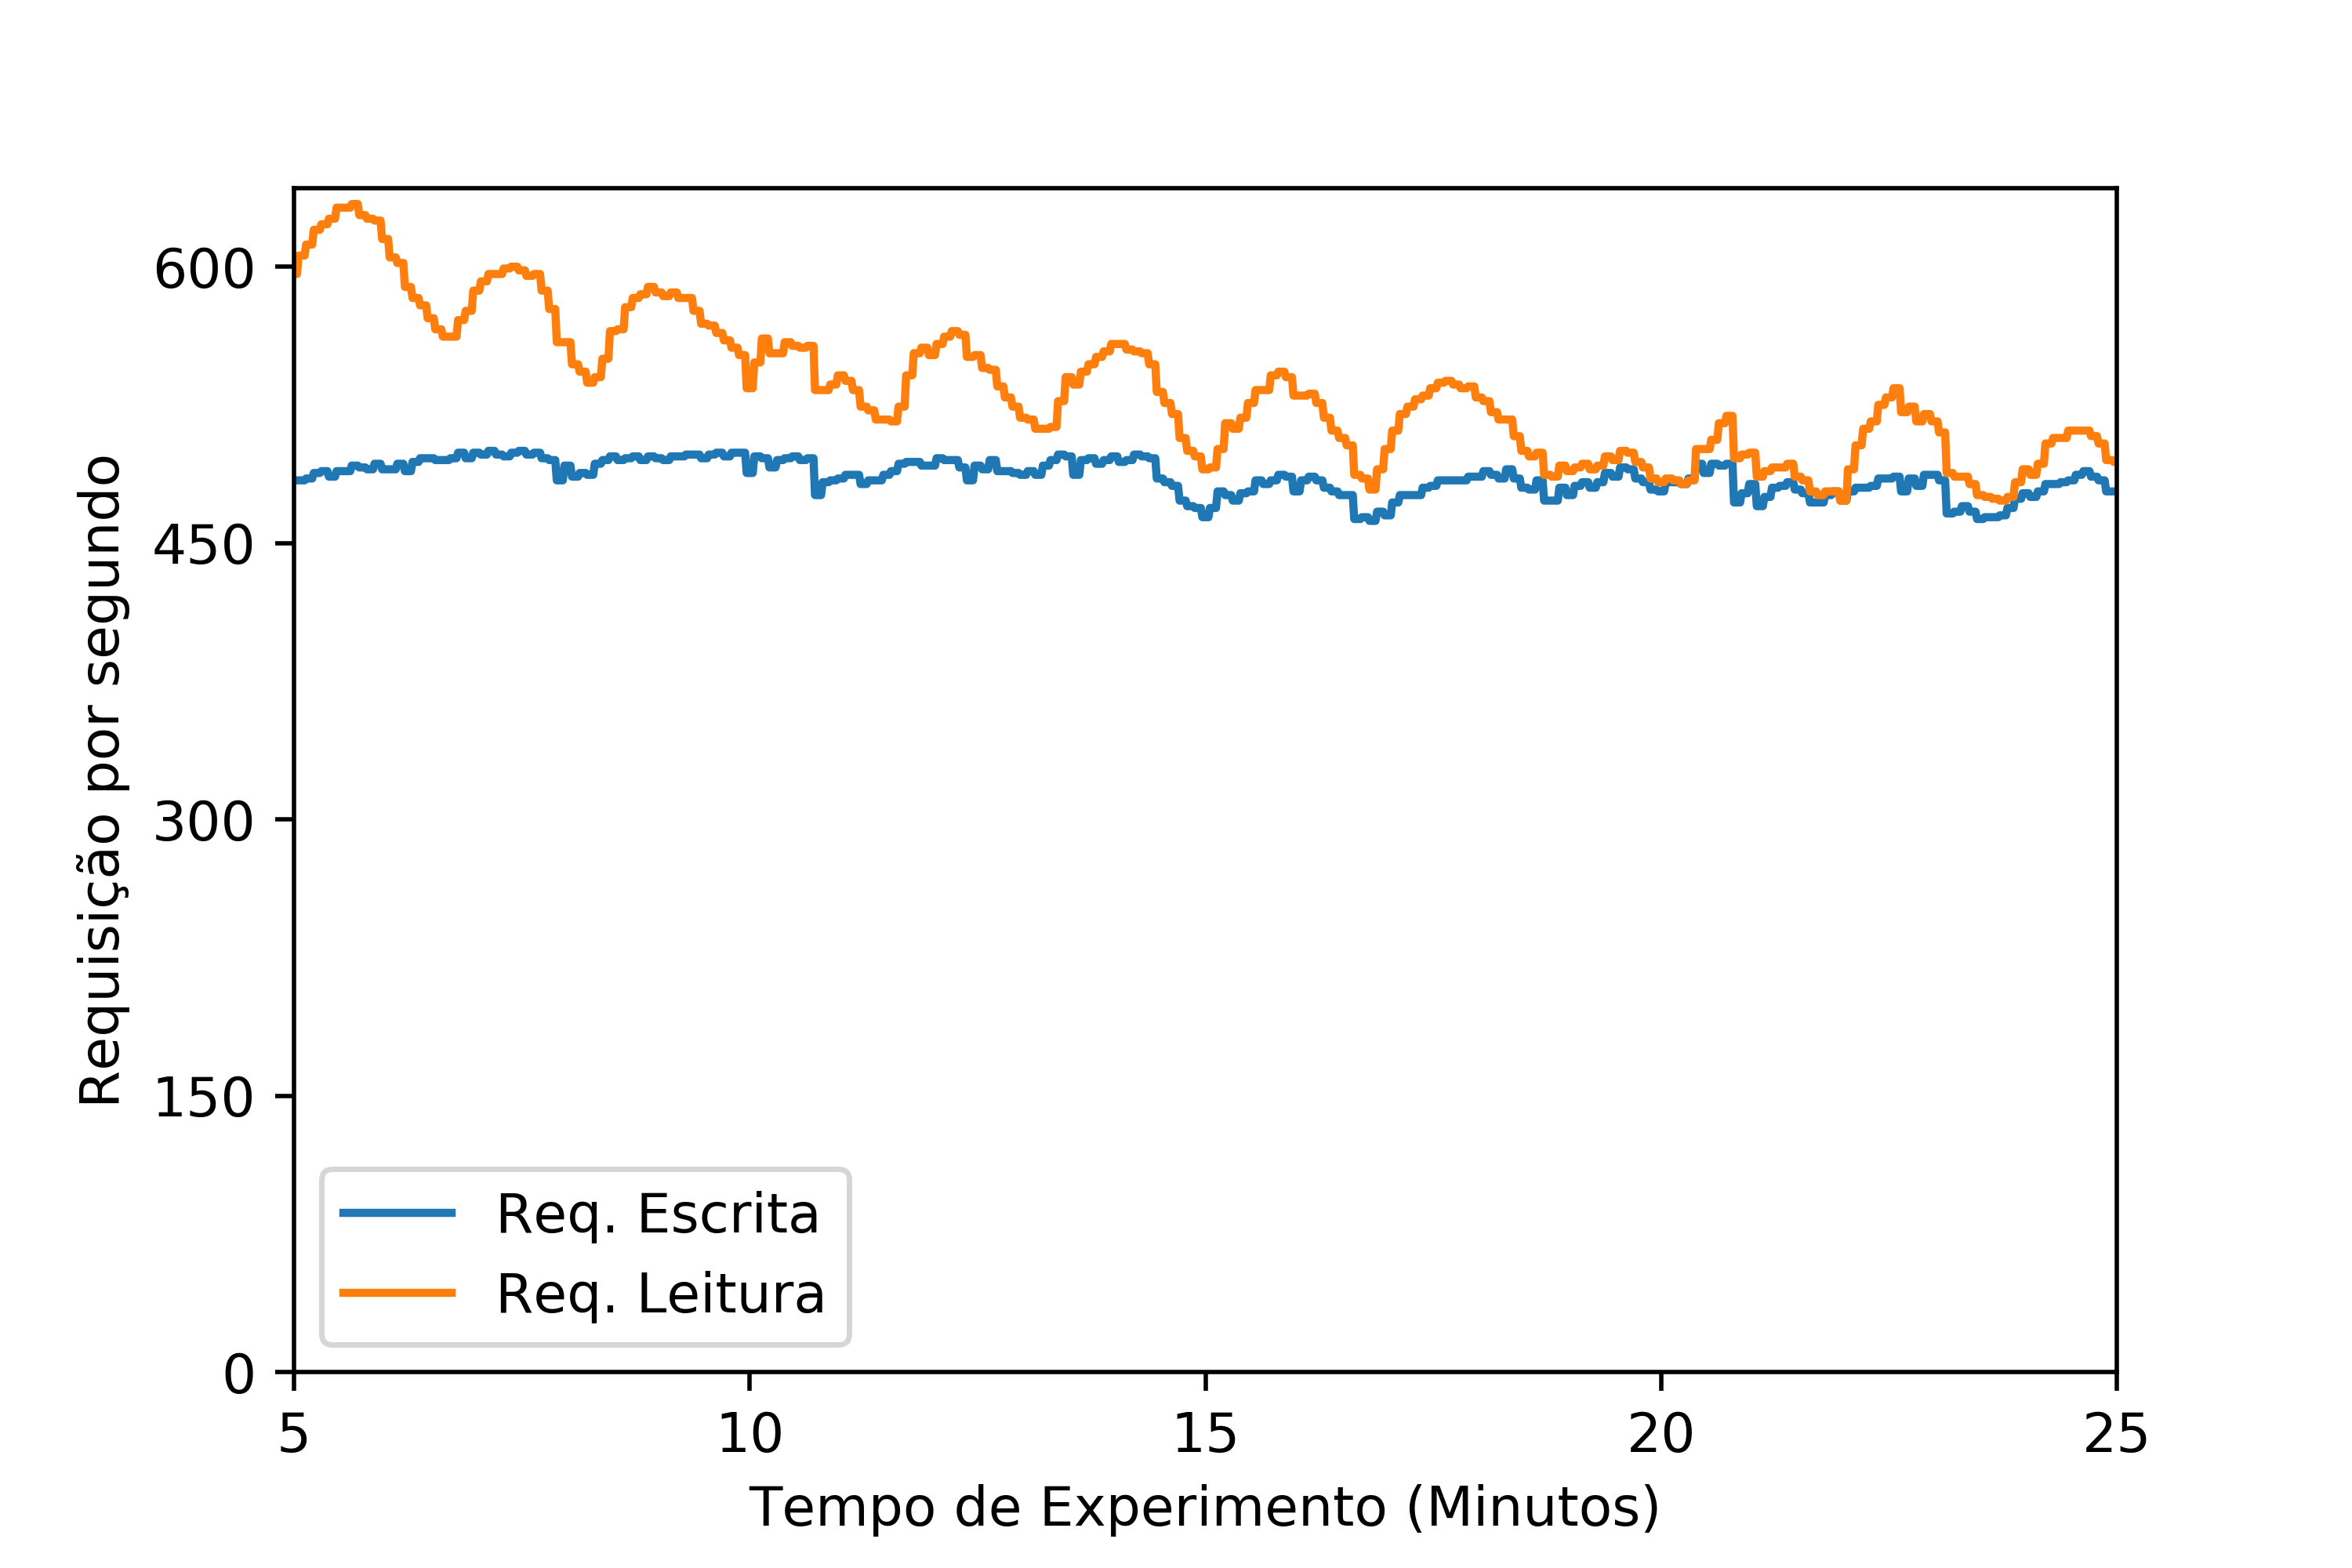
\includegraphics[width=0.5\textwidth]{PI3__RPS__READ-WRITE__LATENCIAS__500W-1500R.png}}
  \caption{Latências e requisições por segundo de escrita e leitura no período de execução de 25 minutos desconsiderando os 5 iniciais do simulador.}
  \label{fig:avr-memmap3}
\end{figure}

\section{Conclusão} \label{sec:conlusao}

De acordo a seção anterior, a Raspberry Pi 3 mostrou-se eficiente nos cenários propostos, alcançando boas respostas em latência, dado que ao observar os resultados em percentil 95 se mantém entre 500ms e 1.000ms. Observando a média, em todas operações se mantiveram abaixo dos 500ms que, para inúmeras aplicações, torna-se mais que necessário e viabiliza o ajuste de muitas aplicações que podem vir a se enquadrar. Podemos ver que ela atende uma boa demanda de requisições por segundo, mantendo-se em torno de 1.100 operações, que representa uma quantidade de atendimento adequada a uma grande gama de aplicações.

Com tais dados, pudemos demonstrar a capacidade da Raspberry Pi 3 em atender a necessidades de muitas aplicações, suprindo os requisitos exigidos pelo paradigma de névoa, tendo em vista os quatro pontos essenciais da névoa. O trabalho aqui apresentado quantificou um pouco do poder do dispositivo em resposta de latência para aplicações semelhantes aos cenários aqui propostos. Como já demonstrado em outros trabalhos, os quesitos energia e peso também são supridos pelo dispositivo.

Em suma, uma possível aplicação seria como integrante em um sistema de carros autônomos \cite{cars1}, para operações não críticas, porém que dependem de baixa latência e uma grande confiabilidade nos dados, dado que, ao percorrer o caminho da rede, pode haver perca de pacotes. Dessa forma é possível diminuir essa perda e o tráfego na rede, enviando somente dados necessários ajudando no treinamento e controle das plataformas. Semelhantemente, aplicações industriais podem ser viáveis, com a chegada do que chamam de indústria 4.0, que integra o uso de IoT em suas aplicações, de forma a possibilitar o uso da \textit{small board}, mantendo o processamento mais próximo do equipamento assim ganhando uma baixa latência e um pré-processamento dos dados \cite{industry4.0}. 

Porém, o dispositivo apresenta limitações, dado que algumas vezes ele consegue atender uma demanda maior de requisições por segundo, mas logo cai novamente. Ao tentar aumentar a demanda via simulador, ocorre um grande número de falhas o que acaba por atrapalhar a avaliação. Isso, no entanto, não é muito diferente de plataformas mais robustas. Outro fator restritivo é a memória, dado que maioria das \textit{small boards} contam com 1GB. Tendo em vista que tanto o \textit{NDBench} e o Cassandra são aplicações robustas, que disponibilizam uma série de parâmetros para que atuem melhor em cenários específicos, através de técnicas como \textit{tuning}, que não foram exploradas neste trabalho, talvez seja possível obter resultados melhores para certas aplicações.

Como trabalhos futuros, cenários diferentes podem vir a ser testados, além de novas aplicações, sendo possível criar um cenário próximo do gerado pelas empresas \textit{Netflix} e \textit{Facebook}. Teríamos, assim, exemplos tanto de aplicações quanto resultados concretos sobre seu uso atual. Da mesma forma, pode-se explorar aplicações mais restritas a cidades inteligentes e aplicações adequadas à indústria 4.0, como pospostos aqui. Possibilidades são abertas quanto ao próprio \textit{hardware}, como o uso da Raspberry Pi 4\footnote{\url{www.raspberrypi.org/products/raspberry-pi-4-model-b}}, além do aumento horizontal do equipamento, que nos possibilita um \textit{cluster} de Raspberry Pi, pois mesmo com o aumento em número de dispositivos, dado seu tamanho, ele ainda continuaria a atender o paradigma. Porém, estudos sobre seu comportamento devem ser realizados para uma quantificação adequada, até mesmo para verificar se o ganho em desempenho e o aumento em consumo de energia é justificado.

\bibliographystyle{sbc}
\bibliography{sbc-template}

\end{document}
